\documentclass[12pt,a4paper]{report}

\usepackage[margin=2.45cm]{geometry}
\usepackage[T1]{fontenc}
\usepackage[utf8]{inputenc}
\usepackage{lmodern}
\usepackage{setspace}
\setstretch{1.42}
\setlength{\parskip}{0.45em}
\setlength{\parindent}{1.15em}
\usepackage{amsmath,amssymb,mathtools}
\usepackage{booktabs,tabularx,array,longtable}
\usepackage{tikz}
\usetikzlibrary{arrows.meta,positioning,shapes.geometric,calc,fit}
\usepackage{pgfplots}
\pgfplotsset{compat=1.16}
\usepackage{caption}
\usepackage{enumitem}
\usepackage{fancyhdr}
\usepackage[hidelinks]{hyperref}
\usepackage{url}

\setlength{\headheight}{14.5pt}
\pagestyle{fancy}
\fancyhf{}
\fancyhead[L]{\nouppercase{\leftmark}}
\fancyhead[R]{\thepage}
\renewcommand{\headrulewidth}{0.3pt}

\numberwithin{equation}{chapter}
\numberwithin{figure}{chapter}
\numberwithin{table}{chapter}

\setlist[itemize]{topsep=0.3em,itemsep=0.2em}
\setlist[enumerate]{topsep=0.3em,itemsep=0.2em}

\captionsetup{font=small,skip=6pt}

\title{Research for Improving the Planting Efficiency of a Wooden Seed Sowing Machine by Using Vision-Guided Feed-Speed Control and Multi-Factor Model Predictive Optimization}
\author{}
\date{October 2026}

\begin{document}

\begin{titlepage}
\centering
\vspace*{1.6cm}
{\Large Computer Science Manuscript}\\[0.4cm]
{\large System Design and Optimization}\\[2.2cm]
{\LARGE\bfseries Research for Improving the Planting Efficiency of a Wooden Seed Sowing Machine by Using Vision-Guided Feed-Speed Control and Multi-Factor Model Predictive Optimization\par}
\vspace{1.6cm}
{\large Three chapters on sensing, control, and numerical estimation}\\[2.4cm]
\begin{minipage}{0.86\textwidth}
\small
This manuscript proposes two control innovations for a planter that meters irregular wooden seeds, principally hardwood seeds such as acorns. Chapter~3 reports a numerical estimation of the models derived in Chapter~2. It is not a field trial and it does not claim measured plantation results.
\end{minipage}
\vfill
{\large October 2026}
\vspace{1.2cm}
\end{titlepage}

\pagenumbering{roman}
\setcounter{page}{1}

\chapter*{Abstract}
\addcontentsline{toc}{chapter}{Abstract}

Direct seeding of hardwoods is attractive because a machine can place wooden seeds, especially acorns, at a fraction of the cost of planting nursery seedlings. The same seeds defeat the assumptions built into cereal planters. An acorn is heavy, elongated, and variable in diameter. A cell that suits red oak doubles on pin oak and misses on bur oak or black walnut. A ground wheel slips on a slope, a seed box vibrates, and a vacuum level copied from a maize meter either does nothing for a large nut or pulls two small seeds into one cell. Previous electronic meters close a speed loop. Previous laboratory studies optimize vacuum, hole size, or vibration one factor at a time, usually offline. Neither line of work coordinates the input speed of the seeds with the factors of the machine while the lot of seeds is changing.

This manuscript studies that gap as a computer-science problem in system design. Two innovations are proposed and then estimated together.

The first innovation is a vision-guided feed-speed controller. A camera over the throat of the hopper measures occupancy, equivalent diameter, and a bridge index. An outer kinematic law converts ground speed and the target spacing into a seed rate. An inner fuzzy proportional--integral--derivative loop drives the cell-wheel motor. A constraint layer slows the wheel when the bridge index crosses a threshold, which is the action that fixed-gain speed control does not take. The vision computer is separate from the motor computer, because earlier vision meters lost the spacing target when image processing and motor control shared one slow microcontroller.

The second innovation is a multi-factor model-predictive coordinator. At a slower period it chooses vibrator frequency, assist vacuum, and opener depth. Its prediction is a logistic map from seed size, vibration, slip, and depth error onto miss probability, double probability, and spacing scatter. The map is minimized on a small grid subject to actuator limits and a penalty on shaker and vacuum effort. The factor loop is deliberately blind to the vision constraint, so it cannot hide a bad vibration setting behind a slower feed. A passive isolator, enabled with this loop, attenuates terrain vibration in the model.

The two loops are stacked. The factor coordinator sets the mechanical regime. The vision loop trims the input speed inside that regime. Chapter~3 integrates the discrete models over 4{,}000 metering events per case, with a fixed random seed, for pin oak, red oak, bur oak, and a mixed lot, at two ground speeds, with slope and with harsh vibration. On a mild red-oak run the quality-of-feed index moves from 58.6\% under ground drive to 88.2\% with both innovations, and the planting-efficiency index moves from 52.4\% to 87.0\%. On bur oak with slope and a 12~Hz terrain disturbance, quality of feed moves from 20.7\% to 75.4\%. On the disturbed mixed lot the efficiency index rises by about 51 percentage points across repeated draws. The shaker uses more energy when it is actually helping. Under a 16~Hz disturbance the optimizer drops the shaker command from 9~Hz to 3~Hz and relies on isolation, which is a result of the cost, not a hand-written rule. These figures are solutions of the stated models. They rank the designs. They are not a substitute for a bench or field test.

\tableofcontents
\listoffigures
\listoftables

\chapter*{Nomenclature}
\addcontentsline{toc}{chapter}{Nomenclature}

\begin{longtable}{@{}lp{0.72\textwidth}@{}}
\toprule
Symbol & Meaning \\
\midrule
\endhead
$X_t$ & Target in-row spacing (m). Nominal value 0.25~m. \\
$v$ & Ground speed of the machine (m/s). \\
$\lambda^{\star}$ & Target seed input rate, $v/X_t$ (seeds/s). \\
$N_c$ & Number of cells on the singulating wheel. Nominal value 12. \\
$\omega$ & Angular speed of the cell wheel (rad/s). \\
$\eta$ & Cell fill ratio, seeds released per cell passage. \\
$s$ & Longitudinal slip of a ground wheel, dimensionless. \\
$d$ & Equivalent seed diameter (mm). \\
$d_c$ & Cell mouth diameter (mm). Nominal value 24~mm. \\
$f$ & Vibrator frequency command (Hz). \\
$f_{\mathrm{dist}}$ & Terrain disturbance frequency reaching the frame (Hz). \\
$f_{\mathrm{eff}}$ & Frequency experienced by the seed mass (Hz). \\
$f^{\star}$ & Size-dependent agitation frequency that the cost prefers (Hz). \\
$P$ & Assist vacuum at the cell (kPa). \\
$h$ & Opener depth (mm). Target $h^{\star}=30$~mm. \\
$\rho$ & Image occupancy of the hopper throat, in $[0,1]$. \\
$B$ & Bridge index computed from occupancy and diameter spread. \\
$p_m,p_d,p_s$ & Probabilities of a miss, a double, and a single at one cell event. \\
$Q_{\mathrm{f}}$ & Quality-of-feed index (\%): spacings in $(0.5X_t,1.5X_t]$. \\
$I_{\mathrm{mult}}$ & Multiple index (\%): spacings at most $0.5X_t$. \\
$I_{\mathrm{miss}}$ & Miss index (\%): spacings greater than $1.5X_t$. \\
$C_{\mathrm{v}}$ & Precision (\%): coefficient of variation inside the qualified band. \\
$\eta_{\mathrm{E}}$ & Planting-efficiency index (\%): qualified seeds per minute divided by the kinematic target. \\
$T_s$ & Sample period of a loop. Motor 10~ms, vision 50~ms, factors 200~ms. \\
\bottomrule
\end{longtable}

\pagenumbering{arabic}
\setcounter{page}{1}

\chapter{Research on Previous Work}
\label{ch:previous}

A wooden seed, in the sense used throughout this manuscript, is a hardwood tree seed whose mass and shape are those of a nut rather than those of a cereal grain. The working examples are pin oak, red oak, and bur oak acorns, together with the larger class that includes seeds for which a maize cell is simply the wrong tool. Black walnut sits in that larger class. The seeds are wooden in the ordinary mechanical sense: the shell is hard, the diameter varies inside a lot, the shape is elongated, and two seeds readily lock against each other in a throat. A sowing machine for these seeds has to accept a stream of irregular objects, release them one at a time, and put each one at a commanded spacing and a commanded depth while the vehicle moves.

The silvicultural reason for caring about the machine is direct seeding. Planting a nursery seedling is reliable and expensive. Placing the seed itself can cost about a third as much, which is why direct seeding of oak remains attractive for restoration even though rodents, drought, and handling still make the biological result less certain than transplanting \cite{lof2019,grossnickle2012,stanturf2014,fao2020}. The machine does not solve depredation. It does decide whether the seed arrives at the right place, at the right depth, and without a double or a gap. Those are placement questions. They are also control questions, because the input speed of the seeds and the factors of the machine move together as soon as the vehicle speed, the slope, or the seed lot changes.

Cereal planters already have a large technical literature. Electric drives replace the ground wheel \cite{aces2024,he2017,zhao2024}. Vacuum plates are optimized for hole diameter, pressure, and peripheral speed \cite{yazgi2007,karayel2004,singh2005,onal2012}. Vision has been put inside a corn meter \cite{borja2021}. Vibration has been measured on rapeseed drills and connected to the seed-filling angle \cite{wu2022,zhang2024vib}. A review of intelligent cereal seeders describes actuators, rate control, and depth control as separate subsystems and asks for multi-sensor fusion in the future \cite{liu2025review}. Hardwood metering is older and thinner. A pneumatic meter on a no-till planter delivered about 95 to 97 percent of the expected density for pin oak and red oak and failed on bur oak and black walnut \cite{wells1990}. A rotating drum with a single-seed pickup was built because nursery beds of oak could not be sown by hand at a stable spacing \cite{dinkel1991}. Forestry practice also includes cab-selected spot sowing during site preparation \cite{newforest}. None of that work closes a loop from an image of the wooden seeds to the feed speed, and then from the seed-lot statistics to vibration, vacuum, and depth, in one designed system.

This chapter reviews the two bodies of work that the later designs extend, and then writes the problem those designs are required to solve. Section~\ref{sec:tech1lit} reviews feed-speed control. Section~\ref{sec:tech2lit} reviews factor optimization. Section~\ref{sec:problem} states the indices, the coupled decision, and the requirements. The innovations themselves are designed in Chapter~\ref{ch:design} and estimated in Chapter~\ref{ch:estimate}.

\section{Research on feed-speed control}
\label{sec:tech1lit}

\subsection{What the feed speed is asked to do}

Precision metering is a rate-matching problem before it is a shape problem. If the machine travels at speed $v$ and the agronomic spacing is $X_t$, the seed input rate that places one seed on each target is
\begin{equation}
\lambda^{\star} = \frac{v}{X_t}.
\label{eq:lambda}
\end{equation}
A wheel with $N_c$ cells, turning at $\omega$ radians per second, releases seeds at
\begin{equation}
\lambda = \frac{N_c\,\omega}{2\pi}\,\eta,
\label{eq:lambdaomega}
\end{equation}
where the fill ratio $\eta$ is the mean number of seeds that actually leave with each cell. Setting $\lambda=\lambda^{\star}$ and solving for the command gives
\begin{equation}
\omega^{\star} = \frac{2\pi\,\lambda^{\star}}{N_c\,\hat\eta} = \frac{2\pi\,v}{N_c\,X_t\,\hat\eta}.
\label{eq:omegastar}
\end{equation}
Every electronic seed meter in the cereal literature is a different way of making $\omega$ track $\omega^{\star}$ when $v$ changes. The difficulty is that $\eta$ is not a constant for wooden seeds, and $v$ is not known perfectly if it is inferred from a wheel that slips.

Equation~\eqref{eq:omegastar} already shows why input speed and machine factors cannot be tuned apart. The fill ratio depends on how well the cell matches the seed, on whether the mass above the cell is bridged, on vibration, and on vacuum. A controller that treats $\hat\eta$ as a number entered by the operator will run at the wrong speed as soon as the lot changes. A controller that only changes vacuum, and leaves $\omega$ on a mechanical ratio, will change $\eta$ and then miss the spacing because $\lambda$ moved. The rest of this section reviews how far published feed-speed control has gone, and where it stops.

\subsection{Ground-wheel drive and slip}

The classical transmission is a ground wheel, a chain, and a gearbox. The cell wheel is geared so that, with no slip and a nominal fill, Equation~\eqref{eq:omegastar} holds. The construction is simple and it needs no electricity. It fails in a specific way. If the drive wheel turns at $(1-s)v$ rather than at $v$, every spacing stretches by $1/(1-s)$. On a slope or on soft ground the slip $s$ is not a small constant. It varies inside a bout. The operator cannot see it in the spacing until plants emerge, and wooden seeds are often not assessed by emergence for a year.

Slip is the reason electronic drives were introduced on row-crop planters. Hydraulic drives first allowed the rate to be set from the cab and allowed a prescription map. Electric drives then removed the shaft and the chain and put a motor on each meter, which adds individual-row shutoff, curve compensation, and a faster change of population \cite{aces2024}. The same reasoning applies to a single-row hardwood planter, with a harsher slip environment: mine spoil, scarified forest soil, and trails are not prepared seedbeds. Wells and colleagues already ran their hardwood meter at modest speeds, 2.4 to 4.0~km/h, and still had to respect slope \cite{wells1990}. A ground wheel on that terrain is a poor speed sensor.

Zhao and colleagues made the same diagnosis for maize and replaced the wheel with an electronic meter whose shaft speed is computed from the set spacing and the measured forward speed \cite{zhao2024}. Their model is the discrete cousin of Equation~\eqref{eq:omegastar}. They report that a fixed-gain proportional--integral--derivative controller was not enough once forward speed kept changing, which is why they scheduled the gains. The hardware lesson carries over. The gain-scheduling lesson only carries over if the disturbance is speed. For wooden seeds the disturbance is also the shape of the next seed.

\begin{figure}[htbp]
\centering
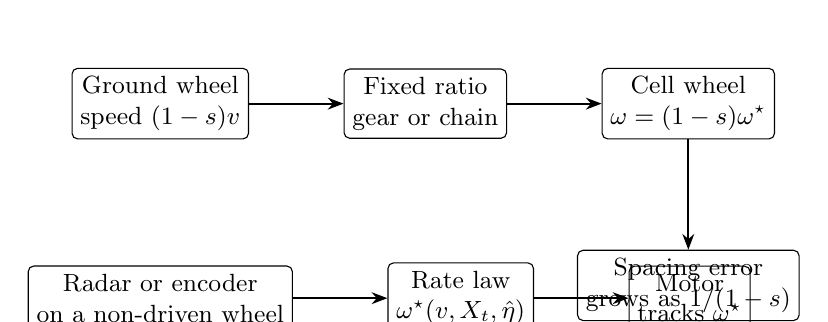
\begin{tikzpicture}[
  font=\small,
  box/.style={draw, rounded corners=2pt, align=center, minimum height=8mm, inner sep=3pt},
  arr/.style={-{Stealth[length=2mm]}, thick}
]
\node[box] (wheel) {Ground wheel\\speed $(1-s)v$};
\node[box, right=12mm of wheel] (gear) {Fixed ratio\\gear or chain};
\node[box, right=12mm of gear] (meter) {Cell wheel\\$\omega=(1-s)\omega^{\star}$};
\node[box, below=14mm of meter] (gap) {Spacing error\\grows as $1/(1-s)$};
\node[box, below=16mm of wheel] (radar) {Radar or encoder\\on a non-driven wheel};
\node[box, right=12mm of radar] (law) {Rate law\\$\omega^{\star}(v,X_t,\hat\eta)$};
\node[box, right=12mm of law] (motor) {Motor\\tracks $\omega^{\star}$};
\draw[arr] (wheel) -- (gear);
\draw[arr] (gear) -- (meter);
\draw[arr] (meter) -- (gap);
\draw[arr] (radar) -- (law);
\draw[arr] (law) -- (motor);
\end{tikzpicture}
\caption{Ground drive copies slip into every spacing. An electronic rate law uses a speed measurement that is not taken from the driven wheel.}
\label{fig:slip}
\end{figure}

\subsection{Proportional--integral--derivative control of the meter shaft}

He and colleagues built a proportional--integral--derivative controller for a maize meter and added integral separation so that a large speed step would not wind the integrator up \cite{he2017}. The plant is the motor and the plate. The setpoint is a plate speed in revolutions per minute. With gains $K_p=16$, $K_i=0.05$, and $K_d=36$ they recorded, for a step from rest to 24~r/min, a rise of about 0.4~s, an overshoot of 1.56 percent, and a steady error of 0.75 percent. On the bench the singulation index reached 98.4 percent at a planting speed of 12~km/h, with multiples and misses not above 1 percent. Those numbers are for graded maize and a plate whose cells match the seed. They show that a well-tuned inner loop can make $\omega$ follow a command. They do not show that the command is the right one when $\eta$ jumps because two acorns have locked in the throat.

The classical tuning route is still the one in Ziegler and Nichols, or a relay experiment, followed by detuning for overshoot \cite{ziegler1942,astrom2006,ogata2010}. For a first-order motor model
\begin{equation}
\tau\dot\omega + \omega = K_m u,
\label{eq:motor1}
\end{equation}
a proportional--integral controller $u = K_p e + K_i\int e$ with $e=\omega^{\star}-\omega$ gives the closed-loop characteristic polynomial
\begin{equation}
\tau s^2 + (1+K_m K_p)s + K_m K_i = 0.
\label{eq:pi-char}
\end{equation}
Both coefficients are positive for positive gains, so the frozen-gain loop is stable. The design knobs are natural frequency and damping, not a table of fuzzy rules. Fuzzy scheduling is useful when the same gains must cover a stick--slip load as the hopper empties, which is the situation Zhao and colleagues addressed \cite{zhao2024}. Their fuzzy proportional--integral--derivative law, tuned from a Ziegler--Nichols start, shortened the simulated response by 0.23~s. On a soil-bin bench the qualified index was 96.74 percent, the multiple index 2.15 percent, and the miss index 1.10 percent. In the field the qualified index fell to 84.21 percent and the miss index rose to 7.89 percent, still inside the industry specification they cite \cite{jb10293}. The drop from bin to field is the number that matters for a forest machine. A controller identified on a smooth belt will meet a rougher disturbance outdoors, and the specification written for maize is not a specification for acorns.

Dambroz and colleagues showed that a low-cost electric drive can also select which seed lot reaches a horizontal disk, and can vary the rate, on a planter type that is common where expensive row drives are not \cite{dambroz2025}. The computer-science content of that machine is a mode switch and a rate command. It is relevant here because a wooden-seed hopper may hold more than one species, as forestry spot sowers already do \cite{newforest}. This manuscript does not design multi-species switching. It does assume that the controller must survive a change of diameter statistics without a new mechanical plate.

\subsection{Machine vision on the meter}

Speed feedback answers the question ``is the shaft turning at $\omega^{\star}$?''. It does not answer ``is there a seed on the next cell?''. Optoelectronic sensors in the seed tube answer a later question: a seed has already been released, or it has not \cite{kocher1998,lan1999,onal2009}. By the time the tube sensor fires, the empty cell has passed the release point. The spacing error is already committed. That is why a camera looking at the plate, rather than at the tube, is the more interesting sensor for feed-speed control.

Borja and colleagues mounted a camera on a pneumatic corn meter and classified each hole as filled or empty \cite{borja2021}. The mechatronic drive advanced the plate when an empty hole was about to be presented, so that a filled neighbour would arrive at the tube on time. The classifier was accurate: 0.2564 percent error on 780 images. At simulated 2 and 4~km/h the vision meter missed significantly less often than the same meter without vision. At 6~km/h the vision meter missed more. The authors attribute the reversal to the microcontroller, which could not finish the image and the motor update inside the time available. The result is a systems result, not an agronomic curiosity. Perception and actuation need separate time budgets. A design that repeats their architecture on a faster wooden-seed wheel will repeat their failure, even if the classifier is perfect.

The image processing they needed is classical. A gray image of a cell can be thresholded by Otsu's method, which chooses the cut that maximises the between-class variance of the histogram \cite{otsu1979,gonzalez2018}. Edges of a seed against the plate can be extracted by Canny's detector when the threshold is unstable \cite{canny1986}. Connected components then yield area $A$, from which an equivalent diameter
\begin{equation}
d = 2\sqrt{\frac{A}{\pi}}
\label{eq:deq}
\end{equation}
is defined even though the seed is not a disk. Circularity $4\pi A/P_{\mathrm{er}}^2$, with $P_{\mathrm{er}}$ the perimeter, is low for an elongated acorn and high for a round pellet. Open-source implementations of these steps are ordinary engineering tools \cite{bradski2000}. A deep detector is not required to decide whether the throat is packed. It would also be the wrong default on a small machine, because the failure mode reported by Borja is latency, and a larger model makes latency worse.

Navid-style image evaluation of a meter on a grease belt is a laboratory cousin of the same idea: the camera grades spacing after the fact \cite{panning2000}. Post-hoc grading is how this manuscript will score its own numerical trials, using the indices of Section~\ref{sec:problem}. It is not a real-time constraint. The real-time use of vision in the first innovation is narrower than a general detector. The camera estimates three scalars---occupancy, mean diameter, and a bridge index---and the constraint layer uses only those scalars. The motor loop never waits for an image.

\subsection{Travel speed as a disturbance, not only as a setpoint}

Equation~\eqref{eq:omegastar} treats $v$ as a known input. Liu and colleagues showed that travel speed also changes the uniformity that a meter can physically deliver \cite{liu2017speed}. Finger-pickup, scoop-wheel, air-pressure, and air-blowing meters for maize were all sensitive to speed, on the bench and in the field. The mechanism is not the control law. At higher peripheral speed the seed has less time to settle in the cell, the release trajectory changes, and bounce in the tube grows. Onal, Degirmencioglu, and Yazgi found an upper seed-release frequency near 16~seeds per second for cotton and maize on their vacuum unit, and an upper peripheral speed near 0.34~m/s, beyond which the qualified index fell \cite{onal2012}. A hardwood planter will not run at maize field speeds. Wells operated near 0.7 to 1.1~m/s. Even in that band, speed remains a disturbance of $\eta$, so a controller that raises $\omega$ in proportion to $v$ can push the cell past the speed at which a heavy seed will still seat.

This is the first place where a pure tracking loop is the wrong optimality condition. Tracking $\omega^{\star}$ minimises $(\omega-\omega^{\star})^2$. Planting efficiency depends on misses and doubles. If raising $\omega$ toward $\omega^{\star}$ increases misses because seeds are bridging, the tracker is faithfully doing harm. The vision constraint in Chapter~\ref{ch:design} exists to break that faithfulness on purpose, for a short time, and then to recover the rate when the bridge index falls.

\subsection{Where feed-speed research stops for wooden seeds}

The reviewed controllers were built for seeds that are small relative to their variation, or that have been graded and coated until they behave like the spherical pellets Yazgi and Degirmencioglu used as a controlled material \cite{yazgi2015}. A wooden seed violates that preparation. Diameter coefficients of variation of 0.12 to 0.20 inside one species, and above 0.30 in a mixed lot, are normal rather than defective. The cell cannot be resized on the move. What can be resized, in effect, is the time allowed for a seed to fall into the cell, and that time is the feed speed.

Published vision adjusts the plate after an empty hole is seen, or grades the result offline. Published fuzzy control adjusts gains so that shaft speed tracks a kinematic command derived from forward speed. Neither computes a bridge index from the shape statistics of the seeds in the throat, and neither treats a reduction of feed speed as a constrained decision rather than as a tracking error. That is the opening for the first innovation. It is an opening in control architecture and in real-time system structure: which computer sees the image, which computer turns the motor, and which quantity is allowed to saturate.

\section{Research on multi-factor optimization}
\label{sec:tech2lit}

\subsection{The factors that actually move the fill ratio}

Feed speed is one input. The machine has others, and the hardwood problem is that they interact. The factors considered in this manuscript are the following.

\begin{enumerate}
\item Vibrator frequency at the seed box. Low-frequency agitation can unlock a bridge of large seeds. High-frequency agitation fluidises a mass of small seeds and, past a threshold, destroys the fill.
\item Assist vacuum at the cell. Vacuum is the main factor in cereal precision meters. For a heavy nut it is a weak force compared with weight, and for a small seed in a large cell it is a way to pick up two seeds.
\item Opener depth. Depth does not change the meter directly. It changes bounce and the vertical error, and it is the factor a forester means by ``sown properly'' \cite{lof2019}.
\item Ground speed, already discussed, which sets the time budget of every other factor.
\item Terrain vibration and slope, which are disturbances rather than commands, but which enter the same equations as the commands.
\end{enumerate}

A design that optimizes one of these while holding the others at a convenient constant will look good in that slice and fail in the slice beside it. The literature is rich in such slices. It is poor in online coordination.

\subsection{Vacuum, hole diameter, and peripheral speed}

Karayel, Barut, and Ozmerzi modelled the vacuum pressure required to hold a seed on a plate as a function of seed mass, hole area, and the speed of the plate \cite{karayel2004}. The force balance is the one every pneumatic meter uses: pressure difference times hole area must exceed weight, centrifugal force, and a margin for vibration. Singh, Singh, and Saraswat optimized pressure, hole size, and speed for cotton and showed that the optimum is a point in a three-dimensional factor space, not a universal pressure \cite{singh2005}. Yazgi and Degirmencioglu made the experimental design explicit. A central composite response surface over vacuum, hole diameter, and peripheral speed, fitted to the multiple index, the miss index, and the quality-of-feed index, gave an optimum near 5.5~kPa and a 3~mm hole for cotton, and no optimum inside the tested range for plate speed \cite{yazgi2007}. The statistical method is appropriate for a fixed seed lot in a laboratory. It produces a setpoint, not a controller. When the next lot has a different diameter, the surface is a different surface, and the machine is already in the field.

The aerodynamic calculation of Onal and colleagues makes the same point from the other direction. A vacuum band that is wide relative to the seed creates a region in which two seeds can seal, so adding holes to a plate in order to lower peripheral speed can raise the multiple index \cite{onal2012}. For maize they recommended the familiar 26-hole plate. For cotton they recommended fewer holes than the 72-hole plate supplied by default. The recommendation is a mechanical redesign. A wooden-seed machine that must accept pin oak and bur oak in the same season cannot carry a family of plates and still claim to be automatic. The online substitute is to change vacuum and feed speed, which are actuators, and to refuse a vacuum that the current diameter statistics do not support. That refusal is exactly what the factor coordinator in Chapter~\ref{ch:design} does when it drives assist vacuum to zero for the lots studied here.

\subsection{Vibration and the seed-filling angle}

Wu and colleagues measured the vibration of a centralized rapeseed meter and reconstructed the seed motion with a discrete-element model \cite{wu2022,cundall1979}. Field frequencies occupied 0 to 180~Hz. In the simulation, vibration did not merely shake seeds in place. It raised the seed-filling angle from a band of 56 to 59 degrees with no vibration to a band of 70 to 91 degrees with vibration. The angle is the geometric expression of how far around the filling zone the seeds are still in contact with the meter. A larger angle means a disturbed free surface. Bench results followed the geometry: with vibration at 10 to 40~Hz the target-seed rate lay between 88.7 and 99.4 percent, against 100 percent with the device at rest. Longitudinal offset of the seed layer mattered more than lateral offset. Holding that offset inside 0 to 20~mm kept the target rate above 91 percent. The practical conclusion they draw is to manage seed-layer height so that vibration has less to act on.

Zhang and colleagues put a hole-wheel rapeseed meter on a rig whose eccentric mass produced controlled vibration, and compared amplitude with frequency \cite{zhang2024vib}. Amplitude, inside a few millimetres, did little. Frequency did a great deal. From 0 to 10~Hz the discharge stayed near 7.6 to 8.2~g/min and the coefficient of variation of uniformity stayed in a stable band. From 10 to 24~Hz the discharge fell nearly linearly with frequency ($R^2=0.92$) and the coefficient of variation rose nearly linearly ($R^2=0.88$). The 10~Hz threshold is the empirical anchor used later in the miss model. It was measured on rapeseed, not on acorns. Using it for wooden seeds is a modelling choice, stated as such in Chapter~\ref{ch:design}, not a claim that an acorn mass has the same resonance. The qualitative content that transfers is the existence of a frequency above which more agitation is not more singulation.

Li and colleagues, working on irregular vegetable seeds rather than on nuts, found the opposite sign at a much higher frequency \cite{li2025drum}. An air-suction drum, with suction near 16~kPa, clearing air near 3.4~kPa, and a cassette vibrated at 50~Hz, reached a qualified rate of 96.9 percent, with 1.4 percent reseeding and 1.7 percent empty holes. Suction dominated, then clearing air, then vibration. The seeds were small and irregular, and the vibration was a high-frequency assist to stop them sticking, not a low-frequency unlock of a bridge of heavy objects. Copying 50~Hz and 16~kPa onto an acorn meter would be a category error. The factor coordinator must be allowed to choose a low frequency for a heavy seed and to choose almost no vacuum when the cell is larger than the seed. A response surface fitted to pepper seeds will not make that choice.

Inclination is a related factor. Lei and colleagues showed that the angle of a centralized rapeseed meter changes the seed motion enough to move the performance indices, using the same discrete-element tools \cite{lei2022,lei2021,hu2021}. A planter on a 10 to 20 degree trail is an inclined meter whether or not the designer intended one. Wells had already included slope in the hardwood tests: pin oak still metered at 97 percent on a 50 percent grade in the laboratory at 3.2~km/h, and red oak at 97 percent on that grade at 4.0~km/h, while the field result on a mild grade was about 95 percent of the target density at 2.4~km/h \cite{wells1990}. The laboratory number and the field number are both high, and both are for the species the cell could accept. The same paper is the source for the failure mode this manuscript refuses to ignore. Bur oak and black walnut did not meter satisfactorily. A larger seed does not become a smaller seed because the vacuum is raised.

\subsection{Mechanical hardwood meters}

The pneumatic hardwood meter of Wells is the closest field ancestor. A commercial no-till unit was rebuilt with a pneumatic singulator and, after penetration failed, with a parabolic ripper. The metering result is species-dependent in exactly the way a fixed cell predicts. Seeds near the design size pass. Seeds far above it do not. There is no vision and no online change of speed beyond the ground-driven ratio.

The Tourney nursery seeder is the closest mechanical ancestor for singulation by geometry rather than by air \cite{dinkel1991}. A drum with an internal pickup carries one acorn out of the mass and releases it at a fixed clock position. Five rows, 26 holes per revolution, a drum speed of 27~r/min at 1~mile per hour, and a target of eight acorns per foot, give a concrete rate calculation of the same family as Equation~\eqref{eq:omegastar}. The inventors abandoned an adjustable cone gearbox for a more direct drive after the gearbox proved to be the wrong place to put the adjustment. That history supports a direct electric drive. It also shows the limit of a purely mechanical pickup: the hole and the clock angle are manufactured, and a mixed lot returns the designer to the original bridging problem they had already seen when several acorns arrived at once.

Maleki and colleagues evaluated a multi-flight auger as a mass-flow meter for a grain drill \cite{maleki2006}. An auger is the wrong singulator for a seed that must be placed at 0.25~m, because it is designed to produce a continuous ribbon. It remains relevant as a warning. Many ``seeders'' in forestry are mass-flow devices or spot broadcasters \cite{newforest}. A precision index is then the wrong score, and a precision controller is the wrong investment. This manuscript is about the precision case: one wooden seed, one station, a measured spacing.

\subsection{Why offline optimization is not a controller}

Response-surface and discrete-element studies share a workflow. The factors are chosen, the machine or the particle model is run, a polynomial or a simulation output is fitted, and an optimum is published. The optimum is a point $(P^{\star}, d_{\mathrm{hole}}^{\star}, \omega^{\star})$ or a recommended band of frequencies. Nothing in that workflow runs while the hopper is emptying and the slope is changing.

Model-predictive control was built for exactly the online version of this workflow. At each sample one solves a finite-horizon problem, applies the first move, and solves again when the state has moved \cite{garcia1989,clarke1987,camacho2007,maciejowski2002,rawlings2017}. Industrial surveys describe the method as standard on slow multivariable plants where constraints are the real specification \cite{qin2003}. The stability theory for the constrained case is mature: a terminal cost and a terminal set, together with a feasible optimisation, give a decreasing cost and an invariant set \cite{mayne2000}. Explicit solutions exist when the problem is a small quadratic program, which removes the need to run an iterative solver on the machine \cite{bemporad2002,boyd2004}. None of this has been the controller of a hardwood meter. Cereal rate loops are single-input speed loops. Cereal factor studies are offline. The second innovation is the transfer of a constrained, receding-horizon coordinator onto the factor vector of a wooden-seed machine, with a prediction model small enough to sit beside the speed loop rather than replace it.

Identification of that prediction model is a separate and older subject \cite{ljung1999,kalman1960,welch1995}. A recursive least-squares update can track a slow change in the gain from frequency to fill as the lot changes. This manuscript uses a fixed logistic map whose coefficients are published in Chapter~\ref{ch:design}, and it says so. The map is structured so that a later project can replace the coefficients with estimates from a bench without changing the coordinator. Pretending that the coefficients are already hardwood measurements would make the estimation in Chapter~\ref{ch:estimate} look like a field result. It is not.

\subsection{Where factor research stops}

Three limits recur.

First, the factors are optimized one experiment at a time. Vacuum studies hold vibration at whatever the bench happens to produce. Vibration studies hold vacuum at the manufacturer's setting. Depth is another control loop in the intelligent-seeder review, often a down-force loop, not a decision variable inside the same cost as miss and multiple \cite{liu2025review}.

Second, the sign of the vibration effect depends on the seed. Rapeseed is hurt above about 10~Hz \cite{zhang2024vib}. Small irregular vegetable seeds are helped at 50~Hz \cite{li2025drum}. Acorn singulation, in the nursery machine, was helped by a geometric pickup and hurt by bridging \cite{dinkel1991}. A coordinator that cannot change its preferred frequency with measured diameter will copy the wrong paper.

Third, the large-seed failure is accepted as a mechanical fact \cite{wells1990}. It is a mechanical fact for a fixed cell and a fixed speed. It is not yet a fact about a machine that is allowed to slow the input, agitate at a few hertz, drop the vacuum, and hold the depth. Whether that combination recovers a useful fraction of the lost quality is the estimation question of Chapter~\ref{ch:estimate}. The literature does not answer it, because the combination has not been the object of the literature.

\begin{figure}[htbp]
\centering
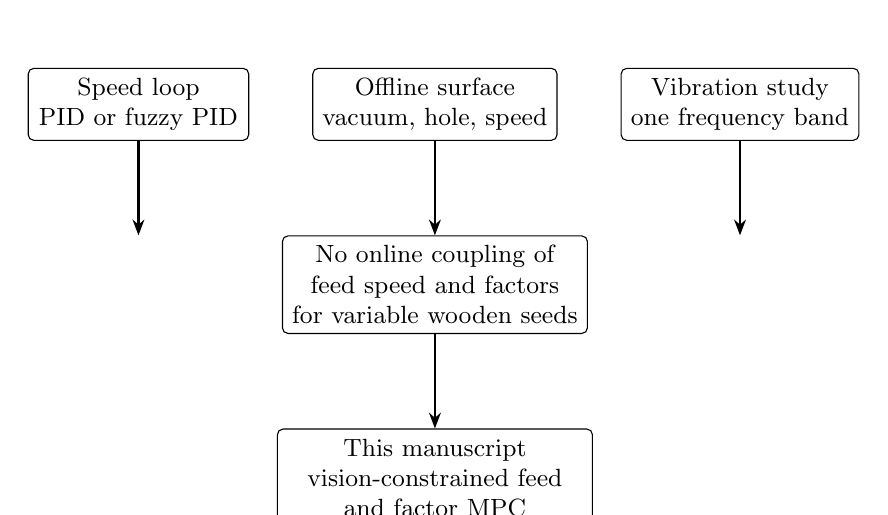
\begin{tikzpicture}[
  font=\small,
  box/.style={draw, rounded corners=2pt, align=center, inner sep=3.5pt, minimum width=28mm},
  arr/.style={-{Stealth[length=2mm]}, thick}
]
\node[box] (lit1) {Speed loop\\PID or fuzzy PID};
\node[box, right=8mm of lit1] (lit2) {Offline surface\\vacuum, hole, speed};
\node[box, right=8mm of lit2] (lit3) {Vibration study\\one frequency band};
\node[box, below=12mm of lit2] (gap) {No online coupling of\\feed speed and factors\\for variable wooden seeds};
\node[box, below=12mm of gap, minimum width=40mm] (new) {This manuscript\\vision-constrained feed\\and factor MPC};
\draw[arr] (lit1.south) -- (gap.north -| lit1.south);
\draw[arr] (lit2) -- (gap);
\draw[arr] (lit3.south) -- (gap.north -| lit3.south);
\draw[arr] (gap) -- (new);
\end{tikzpicture}
\caption{The two research lines stop short of a single online design for irregular wooden seeds. The gap is the problem set of Section~\ref{sec:problem}.}
\label{fig:gap}
\end{figure}

\section{Problem set}
\label{sec:problem}

\subsection{Indices that score a single-seed machine}

Kachman and Smith compared the statistics people report for a precision planter and rejected the bare mean and the bare standard deviation of spacing \cite{kachman1995}. Both are pulled by the misses and the doubles, so a machine with many skips can show a plausible mean. The indices that survived their comparison, and that ISO~7256 and the Chinese single-seed test methods also organise around, are defined from the theoretical spacing $X_t$ \cite{iso7256,gb6973,panning2000}. Let the observed positive spacings be $z_i$. Then
\begin{align}
I_{\mathrm{mult}} &= 100\cdot\frac{1}{n}\#\{i: z_i \le 0.5 X_t\}, \label{eq:imult}\\
Q_{\mathrm{f}} &= 100\cdot\frac{1}{n}\#\{i: 0.5 X_t < z_i \le 1.5 X_t\}, \label{eq:qf}\\
I_{\mathrm{miss}} &= 100\cdot\frac{1}{n}\#\{i: z_i > 1.5 X_t\}. \label{eq:imiss}
\end{align}
The three percentages sum to 100. Precision is the coefficient of variation inside the qualified set only,
\begin{equation}
C_{\mathrm{v}} = 100\cdot\frac{\mathrm{std}\{z_i: 0.5 X_t < z_i \le 1.5 X_t\}}{\mathrm{mean}\{z_i: 0.5 X_t < z_i \le 1.5 X_t\}}.
\label{eq:cv}
\end{equation}
A precision below about 29 to 30 percent is the informal acceptance band cited from Kachman and Smith by later vacuum-meter papers \cite{onal2012}. A miss index and a multiple index each under about 5 percent, and a quality-of-feed index above about 90 percent, are the cereal aspirations. This manuscript does not adopt 90 percent as a pass mark for bur oak. Wells did not get a satisfactory meter on that seed with a fixed pneumatic cell. The problem is to raise the indices from the ground-driven baseline, especially the miss index on large seeds and the multiple index on small seeds, without inventing a new cell for each lot.

Quality of feed is a statement about spacings, not about productivity. A machine that creeps at a low $v$ can post a high $Q_{\mathrm{f}}$ and finish little ground. The planting-efficiency index used in the estimation is the rate of qualified spacings divided by the kinematic target $\lambda^{\star}$:
\begin{equation}
\eta_{\mathrm{E}} = 100\cdot\frac{\text{qualified spacings per second}}{v/X_t}.
\label{eq:eta}
\end{equation}
If the meter runs at the right mean rate and the only errors are local doubles and misses, $\eta_{\mathrm{E}}$ and $Q_{\mathrm{f}}$ are close. If the controller deliberately slows the feed, spacings stretch, $I_{\mathrm{miss}}$ rises, and $\eta_{\mathrm{E}}$ falls even when doubles disappear. That distinction is a required part of the problem statement. A design that only maximises $Q_{\mathrm{f}}$ can do so by going slowly. A design that only maximises seeds per minute can do so by doubling. The cost in Chapter~\ref{ch:design} penalises both.

A short numerical illustration fixes the definitions. Suppose $X_t=0.25$~m and twenty spacings in metres are
\[
\begin{aligned}
&0.04,\ 0.24,\ 0.26,\ 0.23,\ 0.51,\ 0.22,\ 0.25,\ 0.11,\ 0.27,\ 0.24,\\
&0.48,\ 0.25,\ 0.23,\ 0.08,\ 0.26,\ 0.24,\ 0.62,\ 0.25,\ 0.22,\ 0.27.
\end{aligned}
\]
Five spacings are at most 0.125~m, so $I_{\mathrm{mult}}=25$. Three spacings exceed 0.375~m, so $I_{\mathrm{miss}}=15$. The remaining twelve give $Q_{\mathrm{f}}=60$. The qualified values have mean 0.247~m and standard deviation about 0.017~m, so $C_{\mathrm{v}}\approx 6.8$. The mean of all twenty spacings is pulled up by the gaps and would have flattered a bad multiple count if it had been the only report. This is the Kachman argument in one row of numbers. The estimation in Chapter~\ref{ch:estimate} applies the same definitions to thousands of simulated spacings.

\subsection{The coupled decision}

Let the factor command at a slow sample be
\begin{equation}
u_k = \begin{bmatrix} f_k & P_k & h_k \end{bmatrix}^{\mathsf T},
\label{eq:uk}
\end{equation}
and let the fast feed command be the wheel speed $\omega_k$, or equivalently the scale $\sigma_k=\omega_k/\omega^{\star}_k$ by which the kinematic speed is multiplied. The seed lot at that moment is summarised by a diameter distribution with mean $\bar d$ and coefficient of variation $c_d$. Disturbances are slip $s_k$, terrain frequency $f_{\mathrm{dist},k}$, and a depth disturbance. A metering event then produces a spacing contribution whose probabilities depend on all of these:
\begin{equation}
(p_m, p_d, p_s) = \Pi(\bar d, c_d, u_k, \sigma_k, s_k, f_{\mathrm{dist},k}).
\label{eq:pi}
\end{equation}
The map $\Pi$ is specified in Chapter~\ref{ch:design}. The decision problem is to choose the sequence of $u_k$ and $\sigma_k$ so that the expected indices improve and the actuator effort stays inside limits:
\begin{equation}
\begin{aligned}
\min_{u,\sigma}\quad
& \mathbb{E}\big[\, w_m p_m + w_d p_d + w_s (C_{\mathrm{v}}/100) + w_u \ell(u) \,\big] \\
\text{subject to}\quad
& f\in[0,14],\quad P\in[0,8],\quad h\in[15,50],\\
& \sigma\in[0.72,1.08],\quad |\omega_{k+1}-\omega_k|\le \Delta\omega_{\max}.
\end{aligned}
\label{eq:decision}
\end{equation}
The expectation is over the diameter draw and over the disturbances. The weights are design choices. The constraints are hardware limits. Equation~\eqref{eq:decision} is not solved as one giant program on the machine. It is split, and the split is the architecture.

The fast part owns $\sigma$. It can see a bridge forming and it must act inside one or two cell periods. The slow part owns $u$. Vibration, vacuum, and depth are not usefully changed at 100~Hz, and their effect is on the statistics of the next several hundred seeds. Splitting the decision is justified by time scale, which is a standard reason for cascade and hierarchical control \cite{skogestad2005,astrom2008,franklin2019}. It is also justified by failure containment. If the camera stalls, the slow loop still holds a feasible $(f,P,h)$ and the fast loop falls back to kinematic tracking. If the slow solver fails to return a feasible point, the last feasible $u$ is held and the fast loop continues. A single optimiser that needs both the image and a converged quadratic program before it will turn the motor recreates the latency failure of the combined vision meter \cite{borja2021}.

\begin{figure}[htbp]
\centering
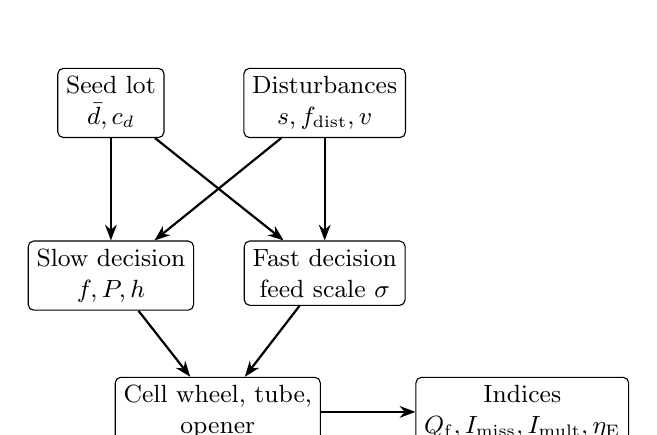
\begin{tikzpicture}[
  font=\small,
  box/.style={draw, rounded corners=2pt, align=center, inner sep=3pt, minimum height=8mm},
  arr/.style={-{Stealth[length=2mm]}, thick}
]
\node[box] (lot) {Seed lot\\$\bar d, c_d$};
\node[box, right=10mm of lot] (dist) {Disturbances\\$s, f_{\mathrm{dist}}, v$};
\node[box, below=13mm of lot] (slow) {Slow decision\\$f, P, h$};
\node[box, below=13mm of dist] (fast) {Fast decision\\feed scale $\sigma$};
\node[box, below=13mm of $(slow)!0.5!(fast)$] (plant) {Cell wheel, tube,\\opener};
\node[box, right=12mm of plant] (score) {Indices\\$Q_{\mathrm{f}}, I_{\mathrm{miss}}, I_{\mathrm{mult}}, \eta_{\mathrm{E}}$};
\draw[arr] (lot) -- (slow);
\draw[arr] (dist) -- (fast);
\draw[arr] (dist) -- (slow);
\draw[arr] (lot) -- (fast);
\draw[arr] (slow) -- (plant);
\draw[arr] (fast) -- (plant);
\draw[arr] (plant) -- (score);
\end{tikzpicture}
\caption{The problem is one plant with two decision rates. Seed-lot statistics and terrain disturbances enter both decisions. The indices are defined on the spacings that leave the plant.}
\label{fig:tworate}
\end{figure}

\subsection{Requirements}

The requirements below are written so that a later bench test can accept or reject the design. The numerical estimation checks only the subset that can be checked on the model.

\begin{enumerate}
\item \textbf{Rate.} Given $v$ and $X_t$, the unconstrained feed command shall implement Equation~\eqref{eq:omegastar} with $\hat\eta=1$ as the nominal fill. The nominal spacing studied here is $X_t=0.25$~m. At $v=1.1$~m/s the target rate is 4.4~seeds/s, or 264~seeds/min.
\item \textbf{Slip.} The speed used in Equation~\eqref{eq:omegastar} shall not be taken from a driven ground wheel. Slope-induced slip shall not scale the mean spacing.
\item \textbf{Bridge constraint.} When the bridge index exceeds its threshold, the feed scale shall decrease, and the decrease shall be limited so that a single bad frame cannot stall the wheel. The limit used in the model is a scale reduction of at most 0.22.
\item \textbf{Latency.} Image features shall be computed on a processor that does not share its deadline with the motor current loop. The motor period is 10~ms. The feature period is 50~ms. A missed feature frame shall hold the last bridge index for at most three periods and then decay the constraint.
\item \textbf{Factors.} Vibration frequency, assist vacuum, and opener depth shall be commands, not factory constants. Frequency shall be selectable at least over 0 to 14~Hz. Vacuum shall be selectable at least over 0 to 8~kPa and shall be allowed to sit at zero.
\item \textbf{Large seed.} On a lot whose mean diameter exceeds the cell, the design shall be scored by the change in $I_{\mathrm{miss}}$ relative to ground drive, not by a maize acceptance threshold.
\item \textbf{Small seed.} On a lot whose mean diameter is well below the cell, the design shall be scored by the change in $I_{\mathrm{mult}}$.
\item \textbf{Harsh vibration.} When the terrain disturbance lies above the 10~Hz anchor, the factor command shall not add a second high frequency on top of it if the predicted miss probability increases.
\item \textbf{Fallback.} Loss of vision shall leave a stable speed loop. Loss of the factor solver shall leave the last feasible factor command.
\item \textbf{Effort.} The cost shall include a positive price on vibrator frequency and on vacuum, so that a flat region of the quality surface does not default to maximum actuation.
\item \textbf{Indices.} Reports shall include $Q_{\mathrm{f}}$, $I_{\mathrm{mult}}$, $I_{\mathrm{miss}}$, $C_{\mathrm{v}}$, and $\eta_{\mathrm{E}}$. A mean spacing alone shall not be used as a pass criterion \cite{kachman1995}.
\item \textbf{Honesty of evidence.} Any number produced by integrating Equation~\eqref{eq:pi} shall be labelled as a model solution. A requirement that needs a physical hopper, a physical camera, or a live seed lot is out of scope for Chapter~\ref{ch:estimate} and remains a requirement on a future experiment.
\end{enumerate}

Requirement~12 is unusual in a problem set and is included because the estimation method can be misread. The logistic map is anchored to published qualitative facts: slip hurts a ground drive \cite{zhao2024,aces2024}; vision can cut misses when the computer keeps up and can fail when it does not \cite{borja2021}; vibration above about 10~Hz hurt the rapeseed meters that were measured \cite{zhang2024vib,wu2022}; vacuum and hole size trade doubles against misses \cite{yazgi2007,onal2012}; large hardwood seeds defeated a fixed pneumatic cell \cite{wells1990}. The coefficients that turn those facts into probabilities are choices of this manuscript. They are published so the estimation can be repeated. They are not identified from a new hardwood experiment.

\subsection{Research questions}

The problem set reduces to three questions, which the remaining chapters answer in design and then in numbers.

\begin{enumerate}
\item Can a feed-speed loop that is allowed to slow down when a vision bridge index is high reduce doubles on small wooden seeds and gaps on large ones, beyond what shaft-speed tracking already achieves by rejecting slip?
\item Can a slow constrained optimiser, choosing vibration, vacuum, and depth from a size-aware prediction, improve the same indices in regimes where speed tracking has little to offer, in particular under terrain vibration and on seeds larger than the cell?
\item When the two loops run together, do they interfere? In particular, does the vision loop's willingness to stretch the spacing cancel the factor loop's gain in planting efficiency, or do the loops improve different terms of the cost?
\end{enumerate}

The first question is about the first innovation. The second is about the second. The third is about the architecture that stacks them. A positive answer to the first two and a qualified answer to the third are both useful. If the stack interferes, the design should say so, because a deployer who turns both loops on by default would otherwise misread the mild-case tables.

\subsection{Scope}

The machine in view is a single-row unit pulled or carried at about 0.7 to 1.2~m/s, with a 12-cell wheel, a 24~mm cell, a vibratory hopper, a small assist vacuum that is allowed to be off, a depth-controlled opener, and a tube. Multi-row coordination, curve compensation, prescription maps, and species switching are outside the design \cite{aces2024,dambroz2025,stafford2000,gebbers2010}. Rodent protection, seed treatment, and germination are outside the indices \cite{lof2019,grossnickle2012}. Communication with a tractor bus is mentioned in the build only as a possible later carrier for the set-point $X_t$; the control design does not depend on ISO~11783 \cite{iso11783}.

The computer-science contribution is the split real-time system, the vision constraint on an otherwise standard motor loop, and the constrained coordinator that treats machine factors as a short-horizon decision with an explicit cost. The mechanical layout in Chapter~\ref{ch:estimate} is the minimum hardware on which those two programs have a meaning. It is not offered as a new singulator geometry. The drum pickup of Dinkel and Kangas and the pneumatic cell of Wells remain the mechanical precedents \cite{dinkel1991,wells1990}. The claim is that those mechanisms are being asked to run open-loop with respect to the two variables that dominate their errors: how fast the wooden seeds are fed in, and how the box, the air, and the opener are set while that happens.

Predictive control enters as a constrained finite-horizon decision, not as a neural policy and not as a claim of global optimality over soil and weather \cite{mayne2000,qin2003}. Fuzzy control enters as a bounded scheduling of three gains on a motor that is already stable at the frozen gains \cite{zadeh1965,mamdani1974,takagi1985,khalil2002}. Vision enters as a scalar constraint, not as a detector of tree species. Each of those reductions is deliberate. Each keeps a failure of one component from becoming a failure of the whole machine, which is the system requirement that the cereal vision meter did not meet when the processor fell behind \cite{borja2021}.

\subsection{How a spacing is measured, and why the index needs a procedure}

The indices of Section~\ref{sec:problem} are only as good as the ruler that produces $z_i$. Three procedures appear in the work reviewed above, and they do not measure the same object.

The sticky-belt procedure lays a belt under the tube, moves the belt at the simulated ground speed, and reads gaps between seeds that have stuck where they fell \cite{panning2000,onal2012,onal2009}. It removes soil bounce and opener depth. It keeps tube bounce and meter errors. It is the right procedure for judging the feed-speed loop, because that loop's product is a release time. ISO~7256 is written in this spirit: a single-seed drill is tested for the regularity of the metered stream, not for the forest that may or may not grow \cite{iso7256}. The Chinese single-seed method GB/T~6973 organises the same three percentages, multiples, qualified, and misses, about the theoretical spacing \cite{gb6973}. JB/T~10293 then turns those percentages into a specification a manufacturer can claim against \cite{jb10293}. A hardwood machine should be willing to be scored by the same arithmetic even if it is not willing to adopt the maize pass marks. The arithmetic is what makes Table~\ref{tab:redmild} comparable with a future belt test.

The field procedure measures plants, not seeds. Emergence, rodents, and depth then enter $z_i$ \cite{lof2019,kachman1995}. A miss in the field is no longer evidence that the cell was empty. Kachman and Smith were explicit that a gap can be a failure to drop or a failure to emerge, and that the indices do not separate them. This manuscript therefore refuses field plant counts as the acceptance test of the controllers. They are the acceptance test of a plantation. Mixing the two is how a good meter is blamed for a dry week, and how a bad meter is excused by a kind season.

The optoelectronic procedure sits between the belt and the field. A gate in the tube times each seed and converts time to distance by multiplying by $v$ \cite{kocher1998,lan1999}. The conversion is exact only if $v$ is the speed used by the kinematic law and the seed's exit velocity along the row is negligible. A heavy acorn leaves the cell with a tangential speed $r\omega$. At $r=0.09$~m and $\omega=2.30$~rad/s that tangential speed is 0.21~m/s, which is not negligible beside a ground speed of 0.7~m/s. The horizontal component depends on the release angle. A tube gate that assumes the seed's row-speed equals $v$ will assign the wrong spacing by a few centimetres, which is enough to move a seed across the 0.5$X_t$ boundary when $X_t=0.25$~m. The estimation avoids that bias by placing seeds from the event model directly. A bench that uses a tube gate will need the release-angle correction derived in Section~\ref{sec:flight}, or it will disagree with the belt for a reason that is geometry rather than control.

Panning and colleagues also remind the reader that a laboratory ranking and a field ranking of planters need not match, even for sugarbeet, which is a far more uniform seed than an acorn \cite{panning2000}. The estimation in this manuscript is a third thing again: a ranking inside a declared model. It is closer to a belt test than to a field test, and it is not a belt test. The procedure that would make it a belt test is the one named at the end of Chapter~\ref{ch:estimate}.

\subsection{Particle forces underneath the factor map}

The logistic map is a summary. The physics it summarises is a contact problem. A discrete-element model represents each seed as a body with a position and a spin, and integrates the contact forces with its neighbours and with the wall \cite{cundall1979}. The normal force is a spring and a damper in the overlap. The tangential force is a spring limited by friction, which is what allows an arch to stand. For two acorns the overlap spring is a crude model of a wooden shell, but the structure of the argument does not depend on the spring law. An arch over the cell stands when the contact normals meet the wall at an angle steeper than the friction cone. Vibration that reverses the contact force for part of each cycle collapses the arch. Vibration that keeps the contacts sliding turns the hopper into a fluid and the cell fills with whatever arrives, including two small seeds.

Wu and colleagues used that style of model to show a filling angle that opens under vibration, and Hu and colleagues coupled it to an airflow solver for a pneumatic rapeseed meter \cite{wu2022,hu2021,lei2021}. The angle is a geometric observable of the same arch. A larger angle means contacts that have walked up the wall. The 10~Hz threshold of Zhang and colleagues is, in this language, the frequency at which the arch no longer reforms between cycles for a small seed \cite{zhang2024vib}. A large wooden seed has a longer contact time and a higher mass, so the frequency at which its arch collapses is lower. Equation~\eqref{eq:fstar} is that statement written as a decreasing function of diameter. It is not a modal analysis of an acorn. It is the smallest formula that gives the coordinator permission to treat pin oak and bur oak as different vibratory problems, which the single-frequency vegetable-seed result does not \cite{li2025drum}.

Inclination enters the same contact balance. On a slope the gravity vector gains a component along the throat, and the arch becomes asymmetric \cite{lei2022}. Wells could still meter red oak on a steep laboratory grade because the pneumatic force dominated that component for a seed that fitted the hole \cite{wells1990}. A seed that does not fit never receives the pneumatic force, and the slope component only makes the miss more likely. The slip term in Equation~\eqref{eq:zm} is the kinematic half of slope. The contact half is left inside the miss coefficient on $\delta_{+}$, which is why the estimation does not add a third slope mechanism. Adding one without a measurement would be a second unsupported constant.

This particle picture also explains a limit of vision. The camera sees the free surface and the seeds in the window. It does not see the contact forces under that surface. The bridge index is a proxy: high occupancy, low circularity, and oversize are the visible correlates of an arch. They will be wrong when an arch stands below a surface that looks open, which is a known hopper failure and a reason the constraint is capped. A capped constraint can be late. An uncapped constraint can stop the machine on a misread surface. The cap at 22 percent is the design's choice of which error is cheaper.


\chapter{Design of the Two Controllers}
\label{ch:design}

This chapter specifies the two innovations at the level of signals, equations, and timing. Section~\ref{sec:visiondesign} designs the vision-guided feed-speed controller. Section~\ref{sec:mpcdesign} designs the multi-factor coordinator and the stack that joins the two. The hardware that gives these signals a physical place is specified in Section~\ref{sec:build}, after the signals are known, so that the build follows the information flow rather than the other way around.

\section{Vision-guided feed-speed control}
\label{sec:visiondesign}

\subsection{Role of the loop}

The feed-speed controller is a cascade with a constraint. The outer input is ground speed $v$ and the spacing set-point $X_t$. The inner output is a motor voltage, or a speed-mode torque command, that turns the cell wheel. Between them sits a scalar $\sigma\in[0.72,1.08]$ that multiplies the kinematic speed. When the throat looks clear, $\sigma$ stays near 1 and the loop is an ordinary electronic meter \cite{he2017,zhao2024}. When the throat looks bridged, $\sigma$ falls and the wheel waits. The waiting is the innovation. A tracker without the constraint would treat the same situation as a brief shortfall of fill and would not change its behaviour at all, because the shaft would still be at the commanded speed.

The loop does not detect species and does not draw boxes around seeds for an operator. It compresses each accepted frame into the features of Section~\ref{sec:features}. Those features are the only vision data the motor computer is allowed to see.

\subsection{Sensing and timing}

Two speed sensors are required by the problem set. A radar, or an encoder on an undriven wheel, supplies $v$. An encoder on the cell-wheel shaft supplies $\omega$. A driven ground wheel is logged and is not used in the control law, so that a later comparison with ground drive remains possible.

The camera looks down at the hopper throat through a window that is wiped mechanically. The region of interest is fixed in the image, about 640 by 200 pixels after cropping, covering the last few centimetres before the cell mouth. The exposure is strobed for 0.2~ms so that motion at 1.2~m/s does not smear a seed by more than a fraction of a millimetre at the working distance. The vision processor runs the steps of Section~\ref{sec:features} and publishes a feature datagram at 20~Hz. The motor computer runs at 100~Hz. If a datagram is late, the motor computer holds the previous bridge index and increments a miss counter. After three missed datagrams, 150~ms, it decays the bridge index by half each further period and the constraint opens. The motor never blocks on a frame. This split is the direct answer to the 6~km/h reversal reported when one microcontroller did both jobs \cite{borja2021}.

A photoelectric sensor in the seed tube is not inside the constraint. It is a logger. It counts releases so that an estimator can compare commanded rate with delivered rate. Using it as the bridge sensor would reintroduce the delay the camera is there to avoid \cite{kocher1998,lan1999}.

\begin{figure}[htbp]
\centering
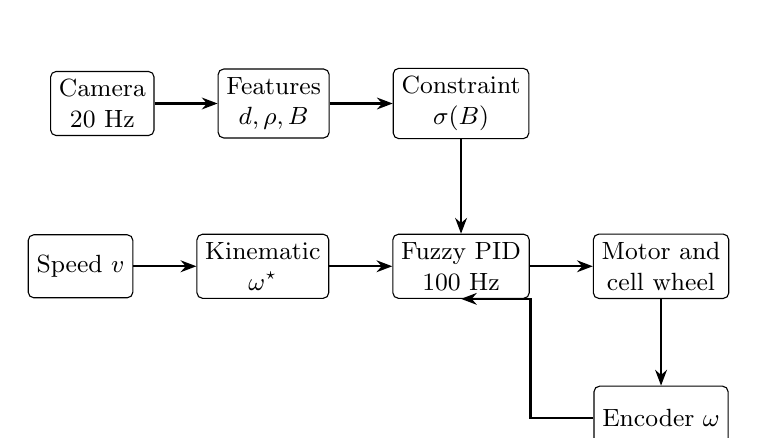
\begin{tikzpicture}[
  font=\small,
  box/.style={draw, rounded corners=2pt, align=center, minimum height=8mm, inner sep=3pt},
  arr/.style={-{Stealth[length=2mm]}, thick}
]
\node[box] (cam) {Camera\\20~Hz};
\node[box, right=8mm of cam] (feat) {Features\\$d,\rho,B$};
\node[box, right=8mm of feat] (con) {Constraint\\$\sigma(B)$};
\node[box, below=12mm of con] (fuzzy) {Fuzzy PID\\100~Hz};
\node[box, left=8mm of fuzzy] (law) {Kinematic\\$\omega^{\star}$};
\node[box, left=8mm of law] (v) {Speed $v$};
\node[box, right=8mm of fuzzy] (mot) {Motor and\\cell wheel};
\node[box, below=11mm of mot] (enc) {Encoder $\omega$};
\draw[arr] (cam) -- (feat);
\draw[arr] (feat) -- (con);
\draw[arr] (con) -- (fuzzy);
\draw[arr] (v) -- (law);
\draw[arr] (law) -- (fuzzy);
\draw[arr] (fuzzy) -- (mot);
\draw[arr] (mot) -- (enc);
\draw[arr] (enc.west) -- ++(-8mm,0) |- (fuzzy.south);
\end{tikzpicture}
\caption{Vision features constrain the speed command. The motor loop closes on the encoder and does not wait for the camera.}
\label{fig:cascade}
\end{figure}

\subsection{Feature extraction}
\label{sec:features}

Each accepted gray frame is normalised by a running estimate of the empty-throat image, so that a slow change of dust does not move the threshold. Otsu's method then separates seed pixels from the background on the residual \cite{otsu1979,gonzalez2018}. Small components, below 20~mm$^2$ at the calibrated scale, are rejected as chips. The remaining components supply areas $A_j$ and perimeters. Equivalent diameters follow Equation~\eqref{eq:deq}. Occupancy is the seed-pixel area divided by the window area,
\begin{equation}
\rho = \frac{1}{A_{\mathrm{win}}}\sum_j A_j.
\label{eq:rho}
\end{equation}
The diameter summary used by the constraint is the mean $\bar d$ of the components and the coefficient of variation $c_d$ of those diameters. Circularity of component $j$ is
\begin{equation}
\gamma_j = \frac{4\pi A_j}{P_{\mathrm{er},j}^2}\in(0,1].
\label{eq:circ}
\end{equation}
An elongated acorn has a low $\gamma_j$. The bridge index combines occupancy, a circularity penalty, and oversize relative to the cell:
\begin{equation}
B = \rho\,(0.45 + 0.55\,\min(1, c_d/0.25))\,\Big(1 + \frac{\max(\bar d - d_c, 0)}{d_c}\Big).
\label{eq:bridge}
\end{equation}
The thresholds inside Equation~\eqref{eq:bridge} are design choices. Occupancy alone would treat a full but flowing throat as a bridge. The circularity term raises the index when the lot is irregular. The oversize term raises it when the seeds in view are larger than the 24~mm cell, which is the bur-oak situation. $B$ is dimensionless. In the numerical model the relief starts at $B>0.42$.

The same frame updates a one-pole filter that the constraint uses as its occupancy state,
\begin{equation}
\rho_{k+1} = 0.92\,\rho_k + 0.08\,\rho^{\mathrm{raw}}_k,
\label{eq:rhofilter}
\end{equation}
so that a single specular frame cannot slam the wheel. When the constraint is active and the wheel has slowed, the raw occupancy target inside the filter is pulled toward 0.48, representing a throat that is being allowed to clear. When the constraint is idle, the filter simply tracks the measurement.

\subsection{Kinematic command and the constraint}

With the nominal fill $\hat\eta=1$ and $N_c=12$,
\begin{equation}
\omega^{\star} = \frac{2\pi v}{12\, X_t}.
\label{eq:wstar2}
\end{equation}
At $v=1.10$~m/s and $X_t=0.25$~m, $\lambda^{\star}=4.40$~seeds/s and $\omega^{\star}=2.304$~rad/s, which is 22.0~r/min. At $v=0.70$~m/s the same spacing asks for 14.0~r/min. These are gentle shaft speeds. The motor is not being asked for maize peripheral speeds. It is being asked for a stable low speed under a changing load, which is a harder control problem than the raw number suggests, because stiction is a larger fraction of the torque.

The constrained command is
\begin{equation}
\omega_{\mathrm{cmd}} = \sigma(B)\,\omega^{\star},
\label{eq:wcmd}
\end{equation}
with
\begin{equation}
\sigma(B) =
\begin{cases}
1, & B \le 0.42,\\[4pt]
1 - \min\big(0.22,\ 0.55\,(B-0.42)\big), & B > 0.42.
\end{cases}
\label{eq:sigma}
\end{equation}
The largest cut is 22 percent. A bridge that would mathematically demand a stop is not allowed to stop the machine. The wheel keeps turning, the tube keeps receiving whatever seeds are free, and the index is recomputed. The lower clip at 0.72 and the upper clip at 1.08 are applied after $\sigma$ and after the small tracking residual of the inner loop, so a noisy fuzzy action cannot wind the scale outside that band.

Equation~\eqref{eq:sigma} is a static nonlinearity, not a second dynamic controller. Its stability effect is that it moves the setpoint. The inner loop is still asked to track a piecewise-constant speed. Setpoint moves are rate-limited at the equivalent of 8~rad/s$^2$ so that a newly detected bridge becomes a ramp rather than a step into the motor.

\subsection{Motor model}

The electrical and mechanical equations of a permanent-magnet direct-current motor, or of a current-controlled brushless motor reduced to the same form, are
\begin{align}
L\frac{\mathrm{d}i}{\mathrm{d}t} &= -Ri - K_e\omega + u, \label{eq:elec}\\
J\frac{\mathrm{d}\omega}{\mathrm{d}t} &= K_t i - b\omega - \tau_{\mathrm{load}}. \label{eq:mech}
\end{align}
The load torque $\tau_{\mathrm{load}}$ contains bearing friction, the intermittent torque of a seed entering a cell, and a stiction term that is largest when the hopper is full. For the speed loop the electrical pole is neglected. It sits well above 100~Hz on a small drive, and the current loop of a servo amplifier already hides it. The design model used for tuning is Equation~\eqref{eq:motor1}, repeated here with the numbers used in the estimation:
\begin{equation}
0.18\,\dot\omega + \omega = u_{\omega},
\label{eq:motornum}
\end{equation}
where $u_{\omega}$ is a speed command in the same units as $\omega$ after the inner current loop, and 0.18~s is the mechanical time constant under a representative hopper load. A 10~ms sample is twenty times faster than this pole, which is the usual rule for a discrete speed loop \cite{franklin2019,ogata2010}.

Load torque is not measured. It appears as a disturbance. Integral action rejects a constant disturbance. A seed that wedges and then releases is a pulse disturbance, which integral action handles if the gains are not so high that the pulse becomes an oscillation. The fuzzy layer exists to lower the proportional gain when the error is large and the error is still growing, and to raise it when the error is small, which is the standard reason for scheduling on a plant whose friction changes \cite{zhao2024,astrom2006}.

\subsection{Discrete fuzzy proportional--integral--derivative law}

Let the sample index of the motor loop be $n$, with $T_m=0.01$~s. The tracking error and its backward difference are
\begin{equation}
e_n = \omega_{\mathrm{cmd},n} - \omega_n, \qquad \Delta e_n = e_n - e_{n-1}.
\label{eq:err}
\end{equation}
The control law is
\begin{equation}
u_n = K_p(e_n,\Delta e_n)\, e_n + K_i(e_n,\Delta e_n)\, T_m\sum_{j=0}^{n} e_j + K_d(e_n,\Delta e_n)\,\frac{\Delta e_n}{T_m},
\label{eq:pid}
\end{equation}
with the integrator clamped and with the sum frozen whenever $|e_n|>e_{\mathrm{sep}}$. The separation threshold used here is $e_{\mathrm{sep}}=0.8$~rad/s. Integral separation is the device He and colleagues used to keep a large step from overshooting, and it is retained for the same reason \cite{he2017}. Anti-windup is the clamp: the summed error is not updated when $u_n$ is on its rail.

The gains are a nominal triple plus a bounded fuzzy increment,
\begin{equation}
K_p = K_{p0}+\Delta K_p,\quad
K_i = K_{i0}+\Delta K_i,\quad
K_d = K_{d0}+\Delta K_d,
\label{eq:gainsplit}
\end{equation}
with $K_{p0}=2.4$, $K_{i0}=6.0$, and $K_{d0}=0.08$ on the normalised speed model of Equation~\eqref{eq:motornum}. The increments are the outputs of a Mamdani inference on two inputs \cite{mamdani1974,zadeh1965}. Each input is scaled into the linguistic range by
\begin{equation}
\tilde e = \mathrm{sat}(e_n/0.6),\qquad \widetilde{\Delta e}=\mathrm{sat}(\Delta e_n/0.15),
\label{eq:scalee}
\end{equation}
where the saturation limits the argument to $[-1,1]$. The linguistic labels are negative big, negative small, zero, positive small, and positive big. Membership of the zero label is a triangle peaking at 0 with support $[-0.4,0.4]$. The small labels are triangles centred at $\pm 0.5$ with support of width 0.8. The big labels are trapezoids that reach membership 1 at $\pm 1$ and fall to 0 at $\pm 0.4$. The same shapes are used for both inputs. Figure~\ref{fig:member} draws the error membership. The increment memberships on the output universe $[-1,1]$ use the same five labels, and the inferred set is reduced to a number by the centroid.

\begin{figure}[htbp]
\centering
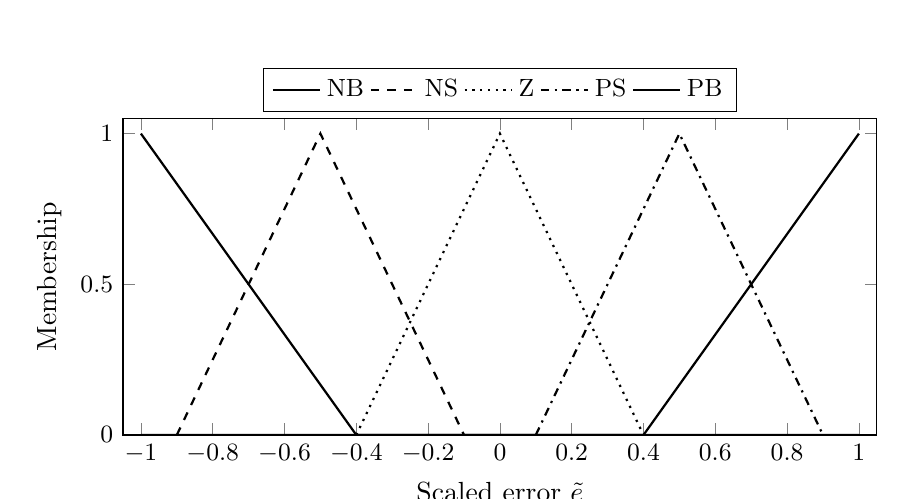
\begin{tikzpicture}
\begin{axis}[
  width=0.92\textwidth, height=5.6cm,
  xlabel={Scaled error $\tilde e$},
  ylabel={Membership},
  xmin=-1.05, xmax=1.05, ymin=0, ymax=1.05,
  legend style={font=\small, at={(0.5,1.02)}, anchor=south, legend columns=5},
  tick label style={font=\small}
]
\addplot[thick] coordinates {(-1,1) (-0.4,0) (1,0)};
\addlegendentry{NB}
\addplot[thick, dashed] coordinates {(-0.9,0) (-0.5,1) (-0.1,0)};
\addlegendentry{NS}
\addplot[thick, dotted] coordinates {(-0.4,0) (0,1) (0.4,0)};
\addlegendentry{Z}
\addplot[thick, dashdotted] coordinates {(0.1,0) (0.5,1) (0.9,0)};
\addlegendentry{PS}
\addplot[thick] coordinates {(-1,0) (0.4,0) (1,1)};
\addlegendentry{PB}
\end{axis}
\end{tikzpicture}
\caption{Membership of the scaled speed error. The same partition is used for the error increment. Output increments use the centroid of the fired labels.}
\label{fig:member}
\end{figure}

Table~\ref{tab:fuzzy} lists the rule for $\Delta K_p$. The rules for $\Delta K_i$ use the opposite corner emphasis: integral gain is allowed to rise only when both the error and the increment are near zero, and it is cut when the error is large, which keeps the separator and the fuzzy layer from fighting. The rules for $\Delta K_d$ raise derivative gain when the error and the increment have the same sign and a large magnitude, that is, when the shaft is running away from the command. Rules are written in the usual condensed form. ``Error is negative big and the increment is negative big implies $\Delta K_p$ positive big'' means the loop is below the command and still falling, so proportional action should strengthen.

\begin{table}[htbp]
\centering
\caption{Rule table for the proportional increment $\Delta K_p$. Rows are the scaled error. Columns are the scaled error increment.}
\label{tab:fuzzy}
\begin{tabular}{@{}lccccc@{}}
\toprule
 & NB & NS & Z & PS & PB \\
\midrule
NB & PB & PB & PS & Z & NS \\
NS & PB & PS & PS & Z & NS \\
Z & PS & PS & Z & NS & NS \\
PS & PS & Z & NS & NS & NB \\
PB & Z & NS & NS & NB & NB \\
\bottomrule
\end{tabular}
\end{table}

The centroid is scaled into the increments by $\Delta K_p \in [-0.8, 0.8]$, $\Delta K_i \in [-2, 2]$, and $\Delta K_d \in [-0.03, 0.03]$. These boxes are part of the design. At every corner, $K_p$ and $K_i$ stay positive, so the proportional--integral polynomial of Equation~\eqref{eq:pi-char} keeps positive coefficients on the design model. A pure derivative $K_d s$ is improper on Equation~\eqref{eq:motornum}. The implementation filters the difference with a first-order pole at 40~Hz, which keeps the high-frequency gain finite \cite{astrom2006}. The resulting claim is limited on purpose. Positive frozen gains and a filtered derivative make each frozen loop a standard stable speed servo on Equation~\eqref{eq:motornum}. They are not a Lyapunov certificate for the time-varying fuzzy system \cite{khalil2002}. The schedule is still reasonable because it moves with the tracking error, and the error of a 0.18~s plant does not cross the whole linguistic range in one 10~ms sample unless the setpoint jumps. Setpoint jumps are rate-limited, as already stated. A vertex check of the discrete spectral radius belongs to the implementation test of a future build. It is not reported as a completed numerical proof in this manuscript.

\subsection{What the constraint does to a spacing sequence}

A cell event occurs every time the wheel advances by $2\pi/N_c$. If the scale $\sigma$ is constant over the event, the distance the machine travels between events is
\begin{equation}
\Delta x = \frac{v}{\lambda} = \frac{X_t}{\sigma},
\label{eq:deltax}
\end{equation}
because $\lambda=\sigma v/X_t$ when the fill is one seed per event. A scale of 0.85 stretches the geometric spacing by $1/0.85\approx 1.18$. Part of that stretch is the point of the constraint: a double that would have produced a 0.2$X_t$ gap is replaced by a later single. Part of the stretch is a new miss if the following event is empty for an unrelated reason. The estimation has to be able to show both parts. A controller that is scored only on doubles will always want the lowest $\sigma$. The efficiency index of Equation~\eqref{eq:eta} punishes the stretch.

The photoelectric count provides a runtime estimate of fill after the fact,
\begin{equation}
\hat\eta_{n} = \frac{N_{\mathrm{tube}}(t_n)-N_{\mathrm{tube}}(t_n-T_{\eta})}{N_c\,(\theta(t_n)-\theta(t_n-T_{\eta}))/2\pi},
\label{eq:etahat}
\end{equation}
with $T_{\eta}=2$~s. This estimate is logged. It is not allowed to divide Equation~\eqref{eq:wstar2} in the present design. Dividing by a noisy $\hat\eta$ rebuilds the kinematic command every two seconds and fights the constraint. A later revision can blend $\hat\eta$ into $\omega^{\star}$ with a time constant of tens of seconds, once a bench has shown that the estimate is calm. The requirement list does not demand that blend.

\subsection{Worked numbers for a red-oak frame}

Take a red-oak mean diameter of 20.5~mm, a lot coefficient of variation of 0.15, and a cell of 24~mm. Suppose the filtered occupancy is 0.62. Equation~\eqref{eq:bridge} gives
\begin{equation}
B = 0.62\,(0.45+0.55\cdot 0.15/0.25)\,(1+0) = 0.62\cdot 0.78 = 0.484,
\end{equation}
because $c_d/0.25=0.60$ and there is no oversize. The excess over 0.42 is 0.064, and $0.55\times 0.064=0.035$, which is below the 0.22 cap. The scale drops from 1 to 0.965. At 1.10~m/s the commanded shaft speed falls from 22.0~r/min to 21.2~r/min. The intervention is small because this frame is only mildly occupied and the seeds fit the cell. That is the correct behaviour. The constraint is not a permanent detune.

Now take a bur-oak frame with $\bar d=32$~mm, $c_d=0.20$, and $\rho=0.70$. Then
\begin{equation}
B = 0.70\,(0.45+0.55\cdot 0.80)\,\big(1+(32-24)/24\big) = 0.70\cdot 0.89\cdot 1.333 = 0.830.
\end{equation}
The excess is 0.410, and $0.55\times 0.410=0.226$, which the cap cuts to 0.22. The scale is 0.78, and the shaft command falls from 22.0~r/min to 17.2~r/min. The wheel gives the large seeds more time. Whether that time becomes filled cells or merely larger gaps is decided by the vibrator as well as by the wheel, which is why the second loop exists. Vision alone, in the later tables, improves doubles more reliably than it improves misses.

\subsection{Fault states inside the feed loop}

Four fault states are defined so that the real-time program has somewhere to go.

\begin{enumerate}
\item \textbf{Vision hold.} A late datagram holds $B$. Tracking continues. A counter is incremented.
\item \textbf{Vision decay.} After 150~ms, $B$ is halved each 50~ms until it lies below 0.42. The constraint opens. The operator lamp for vision is lit. The motor loop is unchanged.
\item \textbf{Encoder loss.} If the shaft encoder misses two periods, the motor current is removed and the wheel stops. Coasting a cell wheel with an unknown speed is how doubles become a pile. This state is a stop, not a fallback to open voltage.
\item \textbf{Speed-sensor loss.} If $v$ is stale for 200~ms, $\omega^{\star}$ is held at its last value for 1~s and then ramped to zero. Holding forever would keep planting after the tractor has stopped only if the failure mode is a stuck high reading, which is unsafe. Ramping down is the chosen failure direction.
\end{enumerate}

None of these states requires the factor coordinator. They are local to the feed computer. The factor computer is informed by a single health bit so that it can freeze $u$ when the wheel is stopped, rather than integrating a model that assumes events are still occurring.

\section{Multi-factor model-predictive optimization}
\label{sec:mpcdesign}

\subsection{Role of the loop}

The factor coordinator owns vibration frequency $f$, assist vacuum $P$, and opener depth $h$. It does not own the wheel speed. It runs at 5~Hz, which is once every 200~ms, and on this machine that is once every few cell events at the speeds of interest. Its job is to keep the triple $(f,P,h)$ at a point where the fast loop's constraint is rarely needed. A coordinator that needs the constraint to look good has chosen a bad regime. For that reason the prediction inside the coordinator is evaluated at $\sigma=1$ and with the vision flag clear. The vision loop may still act, and the estimation credits that action separately. The coordinator is not allowed to assume that the action will happen.

This separation is also a software separation. The factor task can overrun a deadline without stretching a motor period. On an overrun the previous feasible triple is held. Holding a feasible input is the standard fallback of a predictive controller that misses a sample \cite{maciejowski2002,rawlings2017}.

\subsection{Prediction model}
\label{sec:predmodel}

The model is a logistic map from a seed diameter and a factor triple to the probabilities of a miss and a double at one cell event. It is the map $\Pi$ of Equation~\eqref{eq:pi}, written so that it can be evaluated inside a grid search. Define the normalised size errors and the harshness of the motion that the seed mass actually feels:
\begin{align}
\delta_{+} &= \max(d-d_c,0)/d_c, &
\delta_{-} &= \max(d_c-d,0)/d_c, \label{eq:delta}\\
f^{\star}(d) &= \mathrm{clip}\big(4 + 5\, d_c/d,\ 3,\ 11\big), \label{eq:fstar}\\
a(f,d) &= \exp\Big(-\big((f-f^{\star}(d))/2.6\big)^2\Big), \label{eq:agit}\\
H(f_{\mathrm{eff}}) &= \max(f_{\mathrm{eff}}-10, 0)/10. \label{eq:harsh}
\end{align}
The preferred frequency $f^{\star}$ falls as the seed gets larger: a 32~mm seed prefers about 7.8~Hz before the clip, and a 15~mm seed prefers about 12~Hz before the clip, which then limits it to 11~Hz. The Gaussian $a$ is near 1 only when the command sits close to that preference. Harshness $H$ is zero at or below the 10~Hz anchor taken from the rapeseed vibration trials and rises linearly above it \cite{zhang2024vib}. The frequency that enters $H$ is not the command alone. Terrain and the shaker both reach the box,
\begin{equation}
f_{\mathrm{eff}} = \sqrt{\big(\alpha_{\mathrm{iso}} f_{\mathrm{dist}}\big)^2 + f^2}.
\label{eq:feff}
\end{equation}
When the coordinator is off, the isolator is treated as passive and $\alpha_{\mathrm{iso}}=1$. When the coordinator is on, the mount described in Section~\ref{sec:build} is taken to attenuate the terrain contribution to $\alpha_{\mathrm{iso}}=0.55$. That number is an assumption of the model, not a measured transmissibility. It is applied consistently in the estimation, and the text that discusses energy will show what the assumption does: the optimiser can park $f_{\mathrm{eff}}$ just under 10~Hz by a combination of isolation and a modest command.

Depth error, slip, and speed-scale error enter as further dimensionless terms,
\begin{equation}
\varepsilon_h = |h-h^{\star}|/h^{\star},\qquad
o_{\sigma}=\max(\sigma-1.08,0),\qquad
u_{\sigma}=\max(0.92-\sigma,0),
\label{eq:errs}
\end{equation}
with $h^{\star}=30$~mm. The linear predictors are
\begin{align}
\begin{split}
z_m ={}& -1.55 + 5.2\,\delta_{+} + 2.4\,H + 2.6\,s + 2.2\,o_{\sigma} + 1.4\,u_{\sigma} \\
&+ 1.3\,\varepsilon_h - 1.7\,a\,(0.35+\delta_{+}) - 0.85\,\nu\, a,
\end{split} \label{eq:zm}\\
\begin{split}
z_d ={}& -2.05 + 3.6\,\delta_{-} + 1.7\,(P/8)\,(0.4+\delta_{-}) \\
&+ 1.1\,\frac{\max(6-f,0)}{6}\,\delta_{-} + 0.6\,o_{\sigma} - 0.9\,\nu - 0.5\,a.
\end{split} \label{eq:zd}
\end{align}
Here $\nu\in\{0,1\}$ is the vision flag, which the coordinator sets to 0. The probabilities are
\begin{equation}
p_m = \ell(z_m),\qquad
p_d = \ell(z_d)\,(1-p_m),\qquad
p_s = 1-p_m-p_d,
\label{eq:probs}
\end{equation}
with the logistic function $\ell(z)=(1+e^{-z})^{-1}$ evaluated on a clipped $z$ so that the implementation cannot overflow. Scatter of a qualified spacing is modelled as a standard deviation
\begin{equation}
\begin{split}
\varsigma = X_t\Big(&0.07 + 0.045\,H + 0.035\,\varepsilon_h + 0.03\,|\sigma-1| \\
&+ 0.02\,(1-0.6\nu) + 0.015\,|f-f^{\star}|/6\Big).
\end{split}
\label{eq:sigma_scatter}
\end{equation}
Equation~\eqref{eq:sigma_scatter} does not feed the logistic. It feeds the cost, as a stand-in for the precision term.

Each coefficient has a stated job. The intercepts $-1.55$ and $-2.05$ set a mild baseline miss and double probability when every error term is zero and agitation is absent: $\ell(-1.55)\approx 0.175$ and $\ell(-2.05)\approx 0.114$ before the agitation credit, which is then modified by $a$. The large coefficient 5.2 on $\delta_{+}$ is the Wells effect, written as a steep miss penalty once the seed exceeds the cell \cite{wells1990}. The coefficient 3.6 on $\delta_{-}$ is the double penalty for a small seed in a large cell \cite{yazgi2007,onal2012}. The vacuum term is multiplied by $(0.4+\delta_{-})$ so that vacuum is almost harmless when the seed fills the cell and is harmful when the seed is small. The harshness coefficient 2.4 is the Zhang effect, scaled so that a disturbance well above 10~Hz moves the miss probability by tens of points if isolation is absent \cite{zhang2024vib}. None of these coefficients was fitted to a new data set. Replacing them with fitted values is future experimental work. Keeping them public is what makes Chapter~\ref{ch:estimate} repeatable.

\subsection{A numerical evaluation of the map}

The map should be evaluated once by hand so that the later tables have an anchor. Consider red oak at $d=20.5$~mm, $d_c=24$~mm, so $\delta_{+}=0$ and $\delta_{-}=3.5/24=0.1458$. The preferred frequency is
\begin{equation}
f^{\star} = 4 + 5\cdot(24/20.5) = 9.85~\text{Hz},
\end{equation}
inside the clip. With a command $f=9$~Hz,
\begin{equation}
a = \exp\big(-((9-9.85)/2.6)^2\big) = \exp(-0.107) = 0.899.
\end{equation}
Under the coordinator, a terrain frequency of 6~Hz and $\alpha_{\mathrm{iso}}=0.55$ give
\begin{equation}
f_{\mathrm{eff}} = \sqrt{(0.55\cdot 6)^2 + 9^2} = \sqrt{91.89} = 9.59~\text{Hz},
\end{equation}
so $H=0$. Take $\sigma=1$, $s=0.004$, $\varepsilon_h=0$, and $\nu=1$ for a feed-loop evaluation (the coordinator itself would set $\nu=0$). Then
\begin{align}
z_m &= -1.55 + 2.6\cdot 0.004 - 1.7\cdot 0.899\cdot 0.35 - 0.85\cdot 0.899 \nonumber\\
&= -1.55 + 0.010 - 0.535 - 0.764 = -2.84,\\
p_m &= \ell(-2.84) = 0.055.
\end{align}
The double predictor with $P=0$ is
\begin{align}
z_d &= -2.05 + 3.6\cdot 0.1458 - 0.9 - 0.5\cdot 0.899 \nonumber\\
&= -2.05 + 0.525 - 0.9 - 0.450 = -2.87,\\
p_d &= \ell(-2.87)\,(1-0.055) = 0.054\cdot 0.945 = 0.051.
\end{align}
About 89 percent of events at this single diameter are singles before spacing classification. The quality-of-feed index in a full Monte Carlo run is lower than this event-single rate, because spacing classification also punishes rate error, but the event rate shows that the stacked loops sit in a high-single region for a seed that fits the cell.

The contrasting ground-drive evaluation uses $f=0$, $P=3$~kPa, $\nu=0$, $s=0.07$, $\sigma=0.93$, and $f_{\mathrm{eff}}=6$ so that $H=0$. Agitation $a$ is essentially zero because the command is many standard deviations from 9.85~Hz. Then $z_m=-1.55+2.6\cdot 0.07=-1.37$ and $p_m=\ell(-1.37)=0.203$. The double predictor picks up both the size term and the vacuum term,
\begin{equation}
z_d = -2.05 + 0.525 + 1.7\cdot(3/8)\cdot 0.546 + 1.1\cdot 0.146 = -1.02,
\end{equation}
so $\ell(z_d)=0.266$ and $p_d=0.266\cdot(1-0.203)=0.212$. The event-single probability is about 0.58. The ground-drive rows in Chapter~\ref{ch:estimate} land on a quality-of-feed index of the same order. The map is doing what it was constructed to do: a fitted cell without agitation and with a few kilopascals of vacuum doubles a slightly small seed, and wheel slip adds misses.

\subsection{Cost and constraints}

At a coordinator step the diameter distribution is represented by three points, the running mean $\bar d$, the high point $\bar d(1+c_d)$, and the low point $\bar d(1-c_d)$, with weights $1/2$, $1/4$, and $1/4$. The running mean is the vision mean when vision is healthy and a hopper-sample mean entered by the operator otherwise. Using three points rather than a full quadrature is a load decision. The factor computer must finish inside 200~ms with margin, and three evaluations of $\ell$ are cheap.

The cost summed over the three points is
\begin{equation}
J(f,P,h) = \sum_{i=1}^{3} w_i\Big(9\, p_m^{(i)} + 6\, p_d^{(i)} + 4\,\varsigma^{(i)}/X_t + 0.004\, f + 0.01\, P\Big),
\label{eq:cost}
\end{equation}
with $\sigma=1$, $\nu=0$, and the slip inside the prediction fixed at 0.02 because the electronic drive, not the coordinator, is responsible for slip. Depth is not searched. The depth servo is required to hold $h^{\star}$, and the prediction uses $h=h^{\star}$. Searching depth as well would only restate that the best depth error is zero. The servo's value appears in the estimation as a reduction of the depth noise, from a standard deviation of 6.5~mm with a passive opener to 1.2~mm with the servo. That reduction changes $\varepsilon_h$ in Equation~\eqref{eq:zm} and is part of the second innovation's hardware, not a third control algorithm.

The searched set is the Cartesian product
\begin{equation}
f\in\{2,3,\ldots,12\}~\text{Hz by steps of 1},\qquad
P\in\{0, 1, 2, 3.5, 5\}~\text{kPa}.
\label{eq:grid}
\end{equation}
Eleven frequencies and five pressures give 55 costs. Each cost is three logistic evaluations. The search is exhaustive on this set, so the computed minimiser is exact on the set. Exhaustive search on 55 points is a model-predictive controller whose horizon is one statistical step and whose input set is a grid. It is not a long-horizon quadratic program. It is still receding-horizon control in the original sense: the first, and only, move of the solved problem is applied, and the problem is solved again at the next sample with updated $\bar d$ and $f_{\mathrm{dist}}$ \cite{garcia1989,clarke1987}. A one-step horizon is justified because the factor commands have no meaningful dynamics inside 200~ms other than actuator lag, and the lag is handled by a slew limit rather than by a multi-step model. Frequency may change by at most 2~Hz per sample. Vacuum may change by at most 1~kPa per sample. The opener servo has its own loop and is not slewed by this search.

The prices 0.004 on frequency and 0.01 on vacuum are small next to a miss probability of 0.2, which is multiplied by 9. They matter when two grid points have almost the same predicted misses. In that flat region the optimiser prefers the quieter point. Under a harsh terrain disturbance the flat region is not where the action is: adding shaker frequency raises $f_{\mathrm{eff}}$ through Equation~\eqref{eq:feff} and can push $H$ above zero. The price and the harshness term then agree, and the command falls. The estimation shows this fall, from 9~Hz in a mild case to 3~Hz when $f_{\mathrm{dist}}=16$~Hz.

\begin{figure}[htbp]
\centering
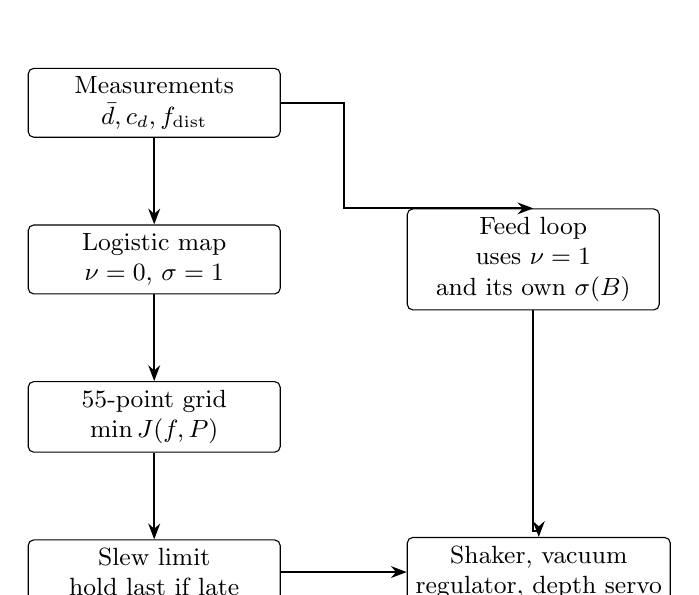
\begin{tikzpicture}[
  font=\small,
  box/.style={draw, rounded corners=2pt, align=center, inner sep=3pt, minimum width=32mm},
  arr/.style={-{Stealth[length=2mm]}, thick}
]
\node[box] (meas) {Measurements\\$\bar d, c_d, f_{\mathrm{dist}}$};
\node[box, below=11mm of meas] (pred) {Logistic map\\$\nu=0$, $\sigma=1$};
\node[box, below=11mm of pred] (grid) {55-point grid\\$\min J(f,P)$};
\node[box, below=11mm of grid] (slew) {Slew limit\\hold last if late};
\node[box, right=16mm of slew] (act) {Shaker, vacuum\\regulator, depth servo};
\node[box, right=16mm of pred] (fast) {Feed loop\\uses $\nu=1$\\and its own $\sigma(B)$};
\draw[arr] (meas) -- (pred);
\draw[arr] (pred) -- (grid);
\draw[arr] (grid) -- (slew);
\draw[arr] (slew) -- (act);
\draw[arr] (meas.east) -- ++(8mm,0) |- (fast.north);
\draw[arr] (fast.south) -- ++(0,-28mm) -| (act.north);
\end{tikzpicture}
\caption{The factor search predicts the meter with vision off. The feed loop then applies the bridge constraint on top of the chosen factors. Neither loop waits for the other.}
\label{fig:hierarchy}
\end{figure}

\subsection{Relation to a quadratic program}

A reader who expects the classical quadratic program can recover it as an approximation. Let $x$ stack the three probabilities and the normalised scatter at the mean diameter, and let the grid be replaced by a box $u\in\mathcal U$. Linearising $\Pi$ about the previous command $u^{-}$ gives
\begin{equation}
x \approx x^{-} + G\,(u-u^{-}),
\label{eq:lin}
\end{equation}
and the cost $9p_m+6p_d+4\varsigma/X_t$ plus a move penalty $(u-u^{-})^{\mathsf T} R (u-u^{-})$ is a convex quadratic if one ignores the logistic curvature, or if one keeps the curvature and accepts a sequential quadratic program \cite{nocedal2006,boyd2004}. Constraints are the box and the slew. That program is the form surveyed by Qin and Badgwell and analysed by Mayne and colleagues \cite{qin2003,mayne2000}. It was not the form implemented for the estimation, because the logistic is cheap to evaluate exactly and the input dimension is two once depth is removed. The grid avoids a linearisation error near $\delta_{+}=0$, where the $\max(\cdot,0)$ terms are not differentiable and a gradient method needs a subgradient convention.

An explicit multi-parametric solution in the sense of Bemporad and colleagues would be attractive if the linear model were trusted, because the control law would become a lookup of critical regions \cite{bemporad2002}. With a non-smooth logistic and an input grid of 55 points, the lookup is the grid itself. Memory on the factor computer is not the binding constraint. Deadline margin is. Fifty-five evaluations leave the processor idle for most of the 200~ms period, which is the desired state of a safety-related task: busy for a short, bounded time, then waiting.

Stability of a one-step constrained search on a static map is simpler than stability of a dynamic horizon. The applied $u$ is always one of the 55 feasible points, the slew limit makes the applied sequence Lipschitz in time, and the plant-side actuators are themselves stable servos. There is no hidden unstable mode in the coordinator. The quality of the closed loop is entirely a question of whether $J$ ranks the true probabilities in the right order. That is a model-quality question, and Chapter~\ref{ch:estimate} does not answer it experimentally. It answers the narrower question of how the indices move when the plant is the same map the coordinator optimises, with Monte Carlo variation of diameter, slip, and depth noise that the coordinator does not see seed by seed. Even in that favourable situation the coordinator is not given the per-seed diameter, only the lot statistics, so the comparison is not a tautology of perfect preview.

\subsection{Information the coordinator is denied}

The following quantities are measured somewhere on the machine and are intentionally not inputs to $J$.

\begin{enumerate}
\item The instantaneous bridge index $B$. If $J$ could see $B$, it would learn to leave a bridge in place and let $\sigma(B)$ clean it up, which shows up as good $p_d$ in a joint predictor and as a poor $\eta_{\mathrm{E}}$ on the machine.
\item The tube count over the last second. That count is the outcome. Using it inside the same period double-counts the event the cost is predicting. A slow outer trim of the intercepts in Equations~\eqref{eq:zm} and \eqref{eq:zd}, with a time constant of a minute, is a reasonable adaptive extension \cite{ljung1999,kalman1960,welch1995}. It is not part of this design.
\item Opener draft force. Draft is a useful depth-loop measurement and a poor miss predictor unless it is calibrated per soil. The depth loop closes on a potentiometer. Draft is logged for a future soil-specific correction.
\end{enumerate}

Denying information is part of the architecture. A hierarchical controller that passes every measurement to every layer becomes a single optimiser with a distributed implementation, and it fails as a single optimiser \cite{skogestad2005}. The bit that does pass upward is health: vision alive, encoder alive, wheel stopped. Health bits change modes. They do not enter $J$ as if they were diameters.

\subsection{Stacking the loops}

The stack at a moment when both loops are healthy is the following sequence. The description is the program order on two computers that share a small datagram and do not share a clock beyond a 1~ms time stamp.

\begin{enumerate}
\item The vision computer publishes $\bar d$, $c_d$, $\rho$, and $B$.
\item The factor computer, if it is on a 200~ms boundary, reads $\bar d$, $c_d$, and the latest inertial estimate of $f_{\mathrm{dist}}$, evaluates $J$ on the grid with $\nu=0$, slew-limits the winner, and publishes $(f,P)$. The depth servo is continuously commanded to $h^{\star}$ and does not wait for this boundary.
\item The motor computer reads $v$ and $B$, forms $\omega_{\mathrm{cmd}}$ from Equations~\eqref{eq:wstar2}--\eqref{eq:sigma}, and runs Equation~\eqref{eq:pid} at 100~Hz.
\item The shaker amplifier and the vacuum regulator track $f$ and $P$ with their own current loops. Those loops are not redesigned here. They are required to reach a 2~Hz step in under 150~ms and a 1~kPa step in under 150~ms, which is the slew assumption made above.
\end{enumerate}

Interference, if it appears, will appear as a gain in $Q_{\mathrm{f}}$ that does not appear in $\eta_{\mathrm{E}}$, because $\sigma<1$ stretches spacings. The problem statement asked for that distinction to be preserved in the report. The estimation therefore publishes both indices for every case, including the cases where vision alone lowers efficiency relative to a pure speed loop. That outcome is a successful warning from the design, not a failure of the table.

\subsection{Parameter summary}

Table~\ref{tab:params} collects the numbers a reimplementation needs. Anything not in the table is a logging choice and does not change the indices.

\begin{table}[htbp]
\centering
\caption{Design parameters used by both the controllers and the numerical estimation.}
\label{tab:params}
\begin{tabular}{@{}llr@{}}
\toprule
Symbol & Role & Value \\
\midrule
$X_t$ & Target spacing & 0.25~m \\
$N_c$ & Cells on the wheel & 12 \\
$d_c$ & Cell mouth & 24~mm \\
$h^{\star}$ & Target depth & 30~mm \\
$T_m$ & Motor period & 10~ms \\
$T_v$ & Vision period & 50~ms \\
$T_f$ & Factor period & 200~ms \\
$\tau$ & Motor time constant & 0.18~s \\
$B_{\mathrm{on}}$ & Constraint threshold & 0.42 \\
$\sigma_{\min}$ & Deepest feed cut & 0.78 \\
$K_{p0},K_{i0},K_{d0}$ & Nominal gains & 2.4,\ 6.0,\ 0.08 \\
$\alpha_{\mathrm{iso}}$ & Terrain attenuation, coordinator on & 0.55 \\
$f_{\mathrm{harsh}}$ & Harshness anchor & 10~Hz \\
Grid & Frequency and vacuum & 11 by 5 points \\
Weights & $p_m$, $p_d$, $\varsigma/X_t$ & 9,\ 6,\ 4 \\
Prices & Per hertz and per kilopascal & 0.004,\ 0.01 \\
\bottomrule
\end{tabular}
\end{table}

The two innovations are now fully specified as programs. The rest of this chapter records the discrete realization, one fully numerical inference, the flight of a seed after release, the schedulability argument, and a slice of the cost grid. The next chapter places the programs on a machine and runs them under the lots and disturbances of the problem set.

\subsection{Discrete realization of the speed loop}
\label{sec:discrete}

Equation~\eqref{eq:motornum} is continuous. The feed computer is not. With a zero-order hold on the command and a sample $T_m=0.01$~s, the exact discretization of $\tau\dot\omega+\omega=u_{\omega}$ is a first-order difference
\begin{equation}
\omega_{n+1} = a\,\omega_n + (1-a)\,u_n, \qquad a = e^{-T_m/\tau}.
\label{eq:discplant}
\end{equation}
Substituting $\tau=0.18$~s gives $T_m/\tau=0.0556$ and $a=0.9460$. The one-step gain on the command is $1-a=0.0540$. A command that steps by 1~rad/s therefore moves the shaft by only 0.054~rad/s on the next sample, which is why the loop needs many samples to finish a bridge-induced ramp and why a 10~ms budget is comfortable for the arithmetic even though it is tight for a stall detector.

The proportional--integral law without the derivative, written backwards in time so that it can be coded as a recurrence, uses the summed error $s_n$ and the clamped increment
\begin{equation}
s_n =
\begin{cases}
s_{n-1}, & |e_n|>0.8~\text{rad/s or } u \text{ on its rail},\\
s_{n-1}+T_m e_n, & \text{otherwise},
\end{cases}
\label{eq:sum}
\end{equation}
and
\begin{equation}
u_n = \mathrm{sat}\big(K_p e_n + K_i s_n + K_d\,\delta_n\big),
\label{eq:usat}
\end{equation}
where $\delta_n$ is the filtered difference. The derivative filter is itself a discrete pole. A continuous pole at 40~Hz has time constant $1/(2\pi\cdot 40)\approx 4.0$~ms. Its exact sample coefficient at 10~ms is not the right object, because the difference is already a once-per-sample quantity. The implementation uses an exponential smoother on $\Delta e_n/T_m$,
\begin{equation}
\delta_n = \beta\,\delta_{n-1} + (1-\beta)\,\frac{e_n-e_{n-1}}{T_m}, \qquad \beta = e^{-T_m/\tau_d},
\label{eq:dfilt}
\end{equation}
with $\tau_d=4$~ms, so $\beta=e^{-2.5}=0.0821$. The filter is fast relative to the motor and slow relative to a single-sample encoder spike. An encoder that glitches by one count on a 4096-count wheel at 22~r/min produces a false $\Delta\omega$ of $2\pi/4096$ radians in 10~ms, which is 0.15~rad/s of false rate. Multiplied by $K_d=0.08$ that glitch is a 0.012~rad/s command bump, smaller than the tracking residual already budgeted in the estimation. The filter is what keeps a two-count glitch from becoming a command. This arithmetic is the sort of check that belongs in the feed computer's design review. It is not a result from a logic analyser.

Integral separation and the rail clamp interact. If the clamp freezes $s_n$ while the separation condition is also true, the sum is frozen once, not twice. The code path must be a single conditional. Two nested conditionals that both subtract the last addition will drift. The specification is Equation~\eqref{eq:sum}: one freeze flag, the logical or of the two reasons.

\subsection{A numerical fuzzy step}

The rule table is easier to trust after one sample is evaluated by hand. Take $e_n=0.30$~rad/s and $e_{n-1}=0.35$~rad/s, so the shaft is below the command and the error is shrinking. The scaled inputs of Equation~\eqref{eq:scalee} are
\begin{equation}
\tilde e = 0.30/0.6 = 0.50, \qquad \widetilde{\Delta e} = (0.30-0.35)/0.15 = -0.333.
\end{equation}
On the error partition of Figure~\ref{fig:member}, $\tilde e=0.50$ sits on the peak of the positive-small triangle, so $\mu_{\mathrm{PS}}(\tilde e)=1$. The positive-big trapezoid is 0 at 0.4 and 1 at 1.0, so
\begin{equation}
\mu_{\mathrm{PB}}(\tilde e) = (0.50-0.40)/(1.00-0.40) = 0.167.
\end{equation}
Zero, negative-small, and negative-big are 0 at this point. On the increment, $-0.333$ falls inside the negative-small triangle centred at $-0.5$ with support from $-0.9$ to $-0.1$. The left slope would be irrelevant. The right slope runs from membership 1 at $-0.5$ to 0 at $-0.1$, and $-0.333$ is $(0.5-0.333)/0.4=0.417$ of the way from the centre to the edge, so $\mu_{\mathrm{NS}}(\widetilde{\Delta e})=1-0.417=0.583$. The zero triangle has support $[-0.4,0.4]$ and peak 1 at 0, so at $-0.333$ its membership is $1-0.333/0.4=0.168$. Negative-big is the trapezoid that is 1 at $-1$ and 0 at $-0.4$. At $-0.333$ it is already 0.

Four rule conjunctions survive, using the minimum for ``and''. From Table~\ref{tab:fuzzy}, error positive-small and increment negative-small fires $\Delta K_p$ at label Z with strength $\min(1,0.583)=0.583$. Error positive-small and increment zero fires NS with strength $\min(1,0.168)=0.168$. Error positive-big and increment negative-small fires NS with strength $\min(0.167,0.583)=0.167$. Error positive-big and increment zero fires NS with strength $\min(0.167,0.168)=0.167$. The output labels are placed at Z$=0$ and NS$=-0.5$ on the increment universe. Aggregating by the maximum, the Z spike has height 0.583 and the NS spike has height $\max(0.168,0.167,0.167)=0.168$. A centroid of two spikes is
\begin{equation}
c = \frac{0.583\cdot 0 + 0.168\cdot(-0.5)}{0.583+0.168} = -0.112.
\end{equation}
Scaled into the proportional box $[-0.8,0.8]$, the increment is $\Delta K_p=-0.090$. The nominal $K_{p0}=2.4$ becomes $K_p=2.31$. The loop is close to the command and the error is already shrinking, so the scheduler slightly reduces proportional gain rather than kicking the shaft. A large growing error would have fired the PB corner of the table and moved $\Delta K_p$ the other way. The example is the ordinary sample, which is the sample the machine sees most often. A design that only behaves well on the linguistic corners and chatters in the middle is the design this calculation is meant to forbid.

The same sample's integral rules, which cut $K_i$ away from zero error, produce a small negative $\Delta K_i$ because $\tilde e$ is not inside the zero label. Derivative rules see an error and an increment of opposite signs, so they do not raise $K_d$. The net command correction relative to the nominal triple is a few percent. That is what ``bounded schedule'' means in a number rather than in a slogan \cite{mamdani1974,takagi1985}.

\subsection{Flight after release}
\label{sec:flight}

The spacing model in the estimation advances the tractor by $X_t/\sigma$ and then adds a random scatter. The scatter has a mechanical source that should be written down so a bench can look for it. A seed leaves the cell at angle $\psi$ below the horizontal with speed $r\omega$ relative to the housing, and the housing moves at $v$. In a frame fixed to the ground at the release instant the initial velocity is
\begin{equation}
\dot x(0) = v - r\omega\cos\psi, \qquad \dot y(0) = -r\omega\sin\psi,
\label{eq:v0}
\end{equation}
with $y$ positive upward and the tube entrance a distance $L_t$ below the release. For the nominal wheel, $r=0.09$~m and $\omega=2.30$~rad/s, so $r\omega=0.207$~m/s. At $\psi=70^\circ$, which is a release on the lower rear of the wheel, $\dot x(0)=v-0.071$~m/s and $\dot y(0)=-0.195$~m/s. The time to fall $L_t=0.40$~m under gravity, ignoring wall strikes, solves
\begin{equation}
L_t = -\dot y(0)\,t + \tfrac12 g t^2.
\label{eq:fall}
\end{equation}
The positive root is $t=0.306$~s when $\dot y(0)=-0.195$~m/s. During that time the tractor moves $vt$. The seed's own $\dot x$ is smaller than $v$ by 0.071~m/s, so the seed lands $0.071\cdot 0.306\approx 0.022$~m behind the point a kinematic model would predict. Two centimetres is 0.09$X_t$. It shifts the whole row. It does not by itself create a miss, because every seed is late by a similar amount when $\omega$ tracks $v$. It creates a miss when $\omega$ and $v$ stop matching, which is exactly the ground-drive slip case, and it creates a double-looking pair when one seed glances off the tube wall and the next does not.

The random term $\varsigma$ in Equation~\eqref{eq:sigma_scatter} is the wall-glance term. Its baseline $0.07X_t=17.5$~mm is the same order as the kinematic lag just computed. The coefficients on harshness and depth add the extra glances that a shaking tube and a bouncing shoe produce. The estimation does not integrate Equation~\eqref{eq:fall} seed by seed. It would be a better bench model and a worse real-time model. The factor computer has no business integrating projectile motion at 5~Hz. The derivation is here so that a disagreement of about two centimetres between a tube gate and a belt is not mistaken for a control failure.

Bounce at the furrow bottom adds a second delay that depth error changes. A seed that strikes a shoe set 10~mm high spends longer in the slot and can roll. The depth servo's job, inside this derivation, is to keep that second delay repeatable. The 1.2~mm residual used when the coordinator is on is a statement that the second delay is then almost common mode and disappears from the spacing differences. The 6.5~mm residual used otherwise is a statement that it does not.

\subsection{Response times of the two computers}

The periods in Table~\ref{tab:params} are not a schedule until each task's worst-case execution is set against them. The feed computer has one control task. At a 2~ms budget inside 10~ms its utilization is 0.20. A single task at that utilization cannot miss a deadline unless the budget is a lie. The stall rule, two missed periods, is then a watchdog on the lie: if the timer interrupt is late twice, the motor current is removed. The watchdog is a hardware timer that the control task must kick. A software counter inside the late task will not count.

The vision and factor computer has two periodic tasks on one processor. Vision needs up to 30~ms every 50~ms. The search needs up to 40~ms every 200~ms. If vision is released first and runs to its budget, the search can start 30~ms into a vision period. In the worst phasing, vision is released again before the search finishes. Preemptive priority is given to vision, so the search is suspended. The search's worst-case response is its own 40~ms plus the vision executions that can preempt it. In 40~ms of search time at most one vision job is released, adding 30~ms, so the response is at most 70~ms. The deadline is 200~ms. The margin is 130~ms, which is the quantity that absorbs a slow frame, a checksum retry, and the logger. This is a response-time bound for two periodic tasks with one preemption edge, not a general schedulability theorem. It is enough for this task set because there are only two tasks and the higher one does not preempt itself.

The bound fails if the vision budget is wrong. A frame that takes 80~ms blows the 50~ms period and steals the margin from the search. The fault rule already treats a late feature datagram as a hold on $B$. The additional requirement is that a frame which overruns is aborted at 30~ms and published as a miss, rather than allowed to complete late and then count as a success. Aborting a late frame is what keeps the 70~ms bound true. Completing it ``just this once'' is how the corn vision meter lost the 6~km/h case \cite{borja2021}.

\begin{figure}[htbp]
\centering
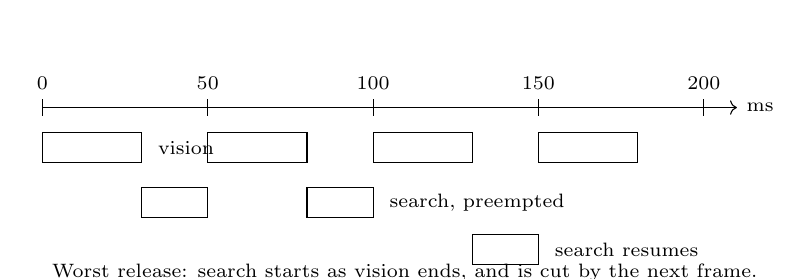
\begin{tikzpicture}[x=0.42mm,y=7mm,font=\scriptsize]
\draw[->] (0,3) -- (210,3) node[right] {ms};
\foreach \x/\lab in {0/0,50/50,100/100,150/150,200/200} {
  \draw (\x,2.85) -- (\x,3.15);
  \node[above] at (\x,3.15) {\lab};
}
\draw (0,2) rectangle (30,2.55);
\node[anchor=west] at (32,2.27) {vision};
\draw (50,2) rectangle (80,2.55);
\draw (100,2) rectangle (130,2.55);
\draw (150,2) rectangle (180,2.55);
\draw (30,1) rectangle (50,1.55);
\draw (80,1) rectangle (100,1.55);
\node[anchor=west] at (102,1.27) {search, preempted};
\draw (130,0.15) rectangle (150,0.7);
\node[anchor=west] at (152,0.42) {search resumes};
\node[anchor=west] at (0,0) {Worst release: search starts as vision ends, and is cut by the next frame.};
\end{tikzpicture}
\caption{Worst-case phasing used for the 70~ms response bound. Vision (top) preempts the factor search (bottom). The search still finishes inside the 200~ms deadline.}
\label{fig:schedule}
\end{figure}

\subsection{A slice of the cost grid}

The search is small enough that a slice of it can be printed. Table~\ref{tab:grid} evaluates Equation~\eqref{eq:cost} at the nominal red-oak diameter 20.5~mm with coefficient of variation 0.15, terrain frequency 6~Hz, slip 0.02, vision flag 0, and the predictor's terrain weight. The predictor does not use $\alpha_{\mathrm{iso}}=0.55$. It uses
\begin{equation}
f_{\mathrm{eff}} = \sqrt{0.35\,f_{\mathrm{dist}}^2 + f^2},
\label{eq:feffpred}
\end{equation}
which is a terrain coefficient $\sqrt{0.35}\approx 0.59$, slightly more pessimistic than the plant coefficient 0.55. The pessimism is intentional in the script that produces Chapter~\ref{ch:estimate}: the search plans for a worse mount than the plant applies. The difference is small. It is recorded here so that a reader who recomputes $f_{\mathrm{eff}}$ with 0.55 and does not match a grid point knows which constant moved.

\begin{table}[htbp]
\centering
\caption{Predicted cost $J$ for nominal red oak at a 6~Hz terrain frequency. Lower is better. Vacuum is in kPa and frequency in Hz.}
\label{tab:grid}
\begin{tabular}{@{}lrrrrr@{}}
\toprule
$f$ & $P=0$ & $P=1$ & $P=2$ & $P=3.5$ & $P=5$ \\
\midrule
3 & 3.052 & 3.157 & 3.267 & 3.443 & 3.631 \\
6 & 2.844 & 2.942 & 3.046 & 3.213 & 3.394 \\
9 & 2.171 & 2.255 & 2.346 & 2.494 & 2.657 \\
12 & 3.219 & 3.300 & 3.387 & 3.529 & 3.685 \\
\bottomrule
\end{tabular}
\end{table}

Every row prefers $P=0$. The vacuum term in Equation~\eqref{eq:zd} has no benefit at $\nu=0$ for this diameter, and the price 0.01 per kilopascal makes a useless vacuum strictly worse. The best printed point is 9~Hz and 0~kPa, with $J=2.171$. Twelve hertz is worse than 3~Hz because $f_{\mathrm{eff}}$ crosses the 10~Hz anchor: $\sqrt{0.35\cdot 36+144}=\sqrt{156.6}=12.5$~Hz. Nine hertz stays under it: $\sqrt{0.35\cdot 36+81}=9.59$~Hz. The Monte Carlo runs select this same corner for mild red oak, so the printed slice and the long runs agree on the nominal lot.

The harsh slice is a near-tie, and the thesis should say so rather than invent a wide margin. At $f_{\mathrm{dist}}=16$~Hz and $P=0$, the same nominal diameter gives $J(3)=3.052$ and $J(9)=3.052$, equal to three digits, with 9~Hz lower only in the fourth digit ($3.0521$ against $3.0522$). Four hertz and 8~Hz are worse, near 3.10 and 3.12. The agitation credit of sitting on $f^{\star}\approx 9.85$~Hz almost cancels the harshness of pushing $f_{\mathrm{eff}}$ to about 13~Hz. The recorded harsh-case run in Chapter~\ref{ch:estimate} selected 3~Hz because the search sees the sample mean of the drawn diameters, not the nominal 20.5~mm, and because a tie keeps the earlier grid point only when the later point is not strictly smaller. A sample mean a few tenths of a millimetre off nominal is enough to break a tie this close. The design consequence is practical. Under a 16~Hz disturbance the coordinator does not have a deep preference between a quiet command and the preferred agitation. Both beat the middle frequencies. A later bench that measures a true preference should replace the harshness coefficient before anyone treats 3~Hz as a unique optimum.

\subsection{Actuator lag and the slew limit}

The grid writes a step. The shaker and the regulator do not. Each is modelled, for the purpose of the slew numbers only, as a first-order lag
\begin{equation}
\tau_a \dot f_a + f_a = f, \qquad \tau_a \dot P_a + P_a = P,
\label{eq:lag}
\end{equation}
with $\tau_a\le 40$~ms so that a 2~Hz step is 95 percent complete in about 120~ms and a 1~kPa step likewise. The requirement stated in the stacking list was 150~ms. The lag model shows that the requirement is a time-constant requirement of about 40~ms, not a vague ``fast enough''. A shaker amplifier that is fast in current and slow in mechanical stroke will violate it even if the electrical specification looks fine. The stroke is the quantity in Equation~\eqref{eq:feff}.

The slew limit of 2~Hz per 200~ms step is 10~Hz per second, which a 40~ms lag can follow. The limit is therefore not hiding an actuator that cannot keep up. It is preventing the search from chattering between the 3~Hz and 9~Hz near-tie when the sample mean jitters. Without the slew, a mean that wanders by a tenth of a millimetre would bang the shaker between two equally good commands. With the slew, a change from 9~Hz to 3~Hz takes three periods, 0.6~s, which is about two or three cell events at 4.4~seeds/s. The seeds in between see an intermediate frequency. That intermediate is one of the middle frequencies the grid dislikes. The estimation does not simulate the slew. It applies the chosen command for the whole run, because each reported case has constant lot statistics and a constant disturbance. A bout in which the disturbance steps from 6~Hz to 16~Hz would pay a short transient the tables do not contain. The transient is bounded by 0.6~s of travel, about 0.7~m at 1.1~m/s, which is three target spacings. Three spacings are visible on a belt and invisible in a 4{,}000-event mean.

\subsection{Failure modes of the stack}

Table~\ref{tab:fmea} lists the failures that change a command, the detection that is actually implemented by the rules already stated, and the command that remains. A failure with no detection does not belong in a table that pretends to be an analysis. Those failures are listed as undetected on purpose.

\begin{table}[htbp]
\centering
\caption{Failures, the detection the design really has, and the command that remains.}
\label{tab:fmea}
\begin{tabular}{@{}p{32mm}p{38mm}p{62mm}@{}}
\toprule
Failure & Detection & Command that remains \\
\midrule
Late vision frame & Datagram age & Last $B$, then decay after 150~ms \\
Wrong scale factor in the camera & Not detected online & A biased $B$. Caught only by the disk calibration \\
Shaft encoder stop & Two missed periods & Motor current removed \\
Radar stuck at a high speed & Not detected online & $\omega^{\star}$ follows the stuck value. A separate timeout on acceleration would be a revision \\
Late factor search & Deadline at 200~ms & Previous $(f,P)$ \\
Search and plant disagree on $\alpha$ & Not a failure. The 0.35 weight is specified & Search is pessimistic relative to the plant \\
Vacuum transducer offset & Zero check at start only & A drifting offset reintroduces doubles. No in-bout zero \\
Depth potentiometer bias & Rail calibration only & A constant depth bias. Spacing scatter grows through $\varepsilon_h$ \\
Isolator collapse, $\alpha\to 1$ & Only if $f_{\mathrm{dist}}$ on the frame rises and the search reacts & The search sees the harsher frequency and moves $f$ \\
\bottomrule
\end{tabular}
\end{table}

Two rows deserve a longer remark because they are the ones a demonstration could hide. A stuck radar is worse than a dead radar. The dead case is specified: after 200~ms the command is held and then ramped to zero. A stuck high case looks like a healthy sensor that believes the tractor is moving. Seeds are metered onto a machine that is standing still, which piles wooden seeds in one spot. The design as written does not detect this. A revision that compares radar speed with the undriven-wheel encoder, and trips when they disagree by more than 15 percent for half a second, would close it. The revision is named here so that the gap is part of the design record rather than a surprise on the first stationary test.

A camera scale error is the other silent fault. The bridge index moves when the millimetre scale moves, because oversize in Equation~\eqref{eq:bridge} is a ratio of diameters. A scale that reads 10 percent high makes a 22~mm seed look like a 24~mm seed and under-calls the bridge. The disk calibration catches a scale error at service. Nothing catches it after the camera is knocked. A cheap in-bout check is the diameter implied by the tube-gate pulse width, which depends on seed size and not on the camera. The design logs the pulse width and does not compare it. The comparison is a consistent extension of the ``tube gate is a logger'' rule: the logger can audit the camera without entering the constraint. Putting the pulse width inside $B$ would couple a post-release sensor into a pre-release decision and would reintroduce the delay the cascade was built to avoid.

\subsection{Quantization, one cell period, and a two-step horizon}

The shaft encoder sets a floor under the fuzzy loop that the continuous model hides. A 4096-count encoder on the cell shaft has an angular quantum of $2\pi/4096=1.53\times 10^{-3}$~rad. At the 10~ms sample the corresponding speed quantum, if speed is a first difference, is $0.153$~rad/s. The nominal red-oak command is $2.30$~rad/s, so the quantum is 6.7 percent of the command if the difference is taken raw. That is coarser than the 0.012 tracking residual used in the estimation, and it would dominate the fuzzy input $\widetilde{\Delta e}$. The feed computer therefore does not differentiate adjacent samples alone. It fits speed over a window of $N_w=8$ samples, 80~ms, which divides the quantum by 8 and yields a speed quantum of about $0.019$~rad/s, just above the residual and just below the scale of $\Delta e$ that moves a membership from zero to small. Eighty milliseconds is 0.44 of the motor time constant, so the window adds lag of that order. The derivative filter of Equation~\eqref{eq:dfilt} and the window are redundant if both are naive. The specification is that the windowed speed is the feedback $\omega_n$, and the derivative filter runs on the tracking error of that already-windowed speed. A second difference of the raw counts is not computed.

The same 80~ms window is the right size relative to a cell. At $\omega=2.30$~rad/s a 12-cell wheel presents a new cell every $2\pi/(12\omega)=0.228$~s. The vision period, 50~ms, samples the throat about four times per cell. The motor period samples it about 23 times. The factor period, 200~ms, is almost one cell. A constraint that changes $\sigma$ therefore takes effect on the cell that is about to be filled, not on a cell that has already released. This timing is the reason the camera looks at the throat rather than at the tube. A tube gate 0.3~s later, from the flight calculation, reports a cell that the wheel has already left. Four vision samples per cell is also the budget inside which a single aborted frame, the 30~ms abort of the response-time argument, still leaves three frames. The bridge index is a vote across those frames through the one-pole filter of Equation~\eqref{eq:rhofilter}, whose 0.92 coefficient remembers roughly twelve frames. A one-frame lie decays. A real bridge, present for a third of a second, accumulates.

A two-step horizon is the natural objection to the one-step grid. Suppose the disturbance is known to step from 6~Hz to 16~Hz one period from now, and the command is 9~Hz. A two-step search could move toward 3~Hz on this period, arriving as the step arrives, whereas the one-step search waits to see 16~Hz and then slews. The value of that preview is the cost of three spacings of intermediate frequency, which the slew analysis already bounded at about 0.7~m of travel. Preview would save that 0.7~m. It would require a forecast of terrain frequency. The inertial unit's one-second Fourier window is a report of the past second, not a forecast of the next 200~ms. Using it as a forecast would be a model of the ground that this machine does not have. The one-step search is the controller that matches the sensor. A terrain map from a previous pass would justify a two-step, or a longer, horizon, and would be a different study, closer to the prescription maps of variable-rate cereal planting than to a single-row hardwood meter \cite{stafford2000,gebbers2010,liu2025review}.

The small-gain view of the constraint is similar in spirit. The map from $\sigma$ to the next bridge index is not known as a transfer function. What is known is a bound. The scale cannot fall by more than 0.22, and the occupancy filter cannot move by more than 0.08 of its input per vision sample. A scale cut therefore cannot chase its own tail inside one cell period: the wheel slows, the filter moves a small step toward the clear-throat target, and the next $\sigma$ is computed from a $B$ that has not yet fully forgotten the bridge. The loop can oscillate only if $B$ itself oscillates, which a real arch does not do at 20~Hz. The cap and the filter are the small-gain ingredients. They are not a computed gain margin. They are the structural reason a margin is plausible, and they are the knobs a bench would turn if the wheel hunted.

\subsection{Rates and power a builder can check with a stopwatch}

The kinematic numbers are simple enough to audit without the simulator, and they should be audited, because every later index is a fraction of them. At $v=1.10$~m/s and $X_t=0.25$~m the target is $\lambda^{\star}=4.40$~seeds/s, which is 264~seeds per minute and 15{,}840~seeds per hour. A 15~litre hopper holding acorns at a bulk density near 0.6~kg/L holds about 9~kg. Red-oak acorns near 4.6~g give roughly 2{,}000~seeds in a full hopper, which is $2000/4.40\approx 455$~s, or seven and a half minutes, of continuous metering. The hopper is a short-bout vessel on purpose. A refill warning at 15 percent mass fires with a little more than a minute left, which is enough to stop at the end of a pass and not enough to forget. Pin-oak seeds are lighter, so the same mass is more seeds and a longer bout. Bur oak is the opposite. The warning is on mass, not on a seed count, because the load cell does not know the species and the camera's count of the throat is not a count of the hopper.

The shaft speed that serves this rate, with twelve cells and a unit fill, is 22.0~r/min. A builder with a tachometer and an empty throat can command that speed and watch the encoder. The check does not need seeds. If the tachometer reads 22~r/min while the radar reads 1.10~m/s and the set spacing is 0.25~m, Equation~\eqref{eq:wstar2} is implemented. Seeds are what test the fill, not the arithmetic.

The energy proxy can be audited in the same spirit. The script accumulates $0.08\omega^2+0.012 f^2+0.02 P^2$ once per cell event. At the mild red-oak both-mode point, $\omega=2.30$~rad/s, $f=9$~Hz, and $P=0$, one event costs
\begin{equation}
0.08\cdot(2.30)^2 + 0.012\cdot 9^2 + 0 = 0.423 + 0.972 = 1.395,
\end{equation}
which matches the table entry 1.39. The shaker term is 70 percent of the proxy. At the harsh-case command $f=3$~Hz the shaker term falls to $0.012\cdot 3^{2}=0.108$, and the wheel term is unchanged, so the event cost falls near $0.53$, again the order of the harsh-case table. The proxy is not a wattmeter. It is a weighted sum that makes this comparison obvious: the camera and the fuzzy increments do not appear in it, and the shaker does. A builder who later measures current will not reproduce 1.39. A builder who finds that the shaker current is a small fraction of the wheel-motor current has discovered that the prices in $J$ were in the wrong ratio, and should raise the frequency price or lower the wheel weight before trusting the quiet-versus-loud tie. The functional form is the part worth keeping. The coefficients 0.08, 0.012, and 0.02 are placeholders until a current clamp replaces them.

Cell time and computer time meet in one inequality that is worth writing as a release check. A cell period is 0.228~s at the nominal rate. Inside that period the feed computer runs about 23 motor steps, the vision computer owes four frames, and the factor computer owes one search. The sums of the budgets are $23\times 2$~ms, $4\times 30$~ms, and 40~ms, which are 46~ms, 120~ms, and 40~ms. The vision budget sum, 120~ms, fits in 228~ms with 108~ms to spare, but only if the four frames do not stack. They do not stack if each frame is aborted at 30~ms, because $4\times 30=120<228$ and the frames are released 50~ms apart. The inequality $4\times 30~\mathrm{ms}<0.228~\mathrm{s}$ is the release check for the nominal speed. It fails at a shaft speed high enough that the cell period drops below 120~ms, which would be $\omega>2\pi/(12\cdot 0.120)=4.36$~rad/s, or about 42~r/min, corresponding to $v=2.08$~m/s at this spacing. The machine is not specified to run there. The inequality says why. It is the same lesson as the 6~km/h reversal on the corn meter, written as a speed limit that belongs to the vision budget rather than to the agronomy \cite{borja2021}.

\subsection{What an empty cell does to the count}

The rate audit above assumes every cell releases one seed. The indices exist because that assumption fails, and the failure has a counting form that is easy to misread on a display. Suppose that over $N$ cell passages the machine travels $N X_t/\sigma$ and releases $N_s$ singles and $N_d$ doubles, with the rest empty. The number of seeds is $N_s+2N_d$. The number of positive spacings is one less than the number of seeds, which for a long run is essentially $N_s+2N_d$. A double contributes a short spacing and also splits what would have been one interval into two, so it increases the spacing count. A miss contributes no spacing of its own. It lengthens a neighbour. The miss index is therefore not $100(N-N_s-N_d)/N$. That ratio is the empty-cell rate. The miss index is the fraction of observed spacings that exceed $1.5X_t$. If empties arrive in isolation, each empty lengthens one spacing from about $X_t$ to about $2X_t$ and the miss index is close to the empty-cell rate. If two empties arrive together, one spacing of about $3X_t$ replaces two empty cells in the count, and the miss index, which divides by the number of spacings rather than by the number of cells, moves differently from the empty-cell rate. The plantation looks worse. The percentage may rise or fall. The estimation's event model places isolated empties more often than bursts, because each event is drawn independently. A real arch lasts for several cells and would burst. The bridge constraint is the mechanism aimed at that burst: it slows the wheel while $B$ stays high, which is a run of cells rather than one draw. The independent-draw estimation therefore understates the value of the constraint on true arches and overstates the chance that a single slow cell is enough. That bias is a reason the both-mode gain on bur oak in Chapter~\ref{ch:estimate} should be read as a lower bound on what a persistent bridge would give the constraint to do, and as an upper bound on how tidy the resulting spacings would look. Independent draws make tidy tables. Arches make clumps. The controller is designed for the clumps. The table is computed from the draws. Both facts belong in the design record so that a belt test full of clumps is not scored as a refutation of a table that assumed none.

A twenty-cell strip makes the distinction numerical. Write E for an empty cell and S for a single, and ignore doubles. The release pattern
\[
\mathrm{S\,S\,E\,S\,S\,S\,E\,E\,S\,S\,S\,S\,E\,S\,S\,S\,S\,S\,E\,S}
\]
has five empties in twenty cells, an empty-cell rate of 25 percent. The spacings, in units of $X_t$ and dropping the final open end, are approximately
\[
1,\,2,\,1,\,1,\,3,\,1,\,1,\,1,\,2,\,1,\,1,\,1,\,1,\,2.
\]
Fourteen spacings follow. Four of them exceed $1.5$, so the miss index is $4/14\approx 29$ percent, against an empty-cell rate of 25 percent. The denominator shrank, because an empty cell does not create a spacing of its own, and the double empty became one spacing of 3 rather than two entries. A display that shows 25 percent skips from the tube gate, which counts empties, and a display that shows 29 percent miss index from a belt, which counts spacings, are both right. They are not the same statistic. The estimation reports the belt statistic, Equations~\eqref{eq:imult}--\eqref{eq:imiss}. The tube gate in the build reports the empty-cell rate through Equation~\eqref{eq:etahat}. An operator who treats them as one number will ``tune'' a controller that is already consistent. The design keeps them on different computers for that reason, not only for the deadline.

\subsection{What the extra analysis changes}

None of these calculations change the five modes of the estimation. They change what a disagreement with the estimation would mean. A two-centimetre bias is flight, not a bad gain. A tie between 3~Hz and 9~Hz is a flat cost, not a bug in the arg-minimum. A vision overrun that is allowed to finish is a broken response-time bound, not a mysterious rise in misses. The controllers remain the constraint of Equation~\eqref{eq:sigma} and the grid of Equation~\eqref{eq:cost}. The surrounding arithmetic is the part that makes those two equations implementable on the two computers of Section~\ref{sec:build} without confusing their faults with their tuning.


\chapter{System Build and Estimation}
\label{ch:estimate}

The controllers of Chapter~\ref{ch:design} need a machine that can produce their signals and a numerical procedure that can score them without pretending to be a field season. Section~\ref{sec:build} specifies that machine as a system build: mechanics only so far as the signals require, then sensors, computers, timing, and calibration. Section~\ref{sec:estimation} integrates the same models the controllers use and reads the indices defined in Section~\ref{sec:problem}.

\section{System build}
\label{sec:build}

\subsection{What the build is for}

The build is a single-row wooden-seed planter whose information architecture matches Figure~\ref{fig:hierarchy}. It is specified here as an engineering description, not as a fabricated prototype. No mass, no weld, and no photographed assembly is claimed. The description is detailed because a control design that does not name its sensors cannot be implemented, and because several modelling assumptions in Chapter~\ref{ch:design} are assumptions about hardware. The isolator attenuation $\alpha_{\mathrm{iso}}=0.55$, the depth-noise reduction from 6.5~mm to 1.2~mm, and the refusal to take speed from a driven wheel are all build decisions. If a later prototype changes them, the estimation has to be rerun. That dependency is intentional.

The agronomic envelope is the one already used in the hardwood trials and in the direct-seeding review. Forward speed is 0.6 to 1.2~m/s. Target spacing is 0.25~m, which is a restoration spacing rather than a nursery-bed spacing of several seeds per foot \cite{dinkel1991,lof2019}. Target depth is 30~mm, inside the band in which acorns are covered without being buried past their reserves. The cell mouth is 24~mm, chosen as a compromise around red oak and knowingly wrong for pin oak and bur oak. The control system is the means of living with that compromise. A family of interchangeable cells would also work, and would not need this thesis. The build keeps one cell in order to force the controllers to do the work.

\subsection{Mechanical path of a seed}

Seeds sit in a hopper of about 15~litres, enough for a short bout at 4.4~seeds/s without a refill and small enough that the changing head of seeds is a real load disturbance on the wheel. The hopper floor is a short vibratory tray driven by an electromagnetic shaker. The tray discharges into a throat that is the camera's window. Below the window, a 12-cell wheel of 180~mm pitch diameter picks seeds from the throat and carries them to a release at the bottom of the housing. Elastomer inserts in the cells accept a diameter band around 24~mm without machining a new wheel for each species. They do not, and cannot, accept a 32~mm acorn and a 15~mm acorn with equal fill. That is the residual the controllers are scored on.

A low-pressure port opens onto the cell during the rising half of the rotation and is vented before release. The port is the assist vacuum. Its regulator must be able to hold 0~kPa, meaning the port is open to atmosphere, because the cost will select that point for small seeds. A regulator that cannot go to zero is the wrong part, even if its span is otherwise impressive. The maximum used by the grid is 5~kPa, and the hardware stop is 8~kPa, above the grid so that a faulted command still has a relief valve under the cereal pressures that this machine deliberately does not use \cite{karayel2004,li2025drum}.

From the release, a smooth tube of 40~mm inside diameter drops the seed to the opener. The tube is straight enough that a photoelectric gate sees one chord of the seed, and short enough that time of flight at a drop of 0.4~m is under 0.3~s. That delay is why the gate is a logger and not the bridge sensor. The opener is a narrow shoe behind a ripper point, the arrangement Wells adopted after a plain no-till opener failed to penetrate spoil \cite{wells1990}. Depth is set by a linear actuator against a gauge wheel, with a potentiometer on the pivot. A press wheel closes the slot. The press wheel is not controlled. Its load is a spring.

The vibratory tray, the cell wheel, the vacuum port, and the opener are the four actuated elements. Everything else is structure. The structure that matters to the model is the mount between the seed box and the frame. Rubber isolators are specified at the box feet, and the coordinator-on case takes their attenuation of terrain frequency as $\alpha_{\mathrm{iso}}=0.55$ in Equation~\eqref{eq:feff}. The coordinator-off case bypasses the assumption by using $\alpha_{\mathrm{iso}}=1$, which represents either locked mounts or a frame that was never isolated. This is a coarse representation of a transfer function. It is enough to let the cost discover that adding shaker frequency on top of an already harsh frame is expensive in misses. A measured transmissibility would replace the constant 0.55 without a change to the grid search.

\begin{figure}[htbp]
\centering
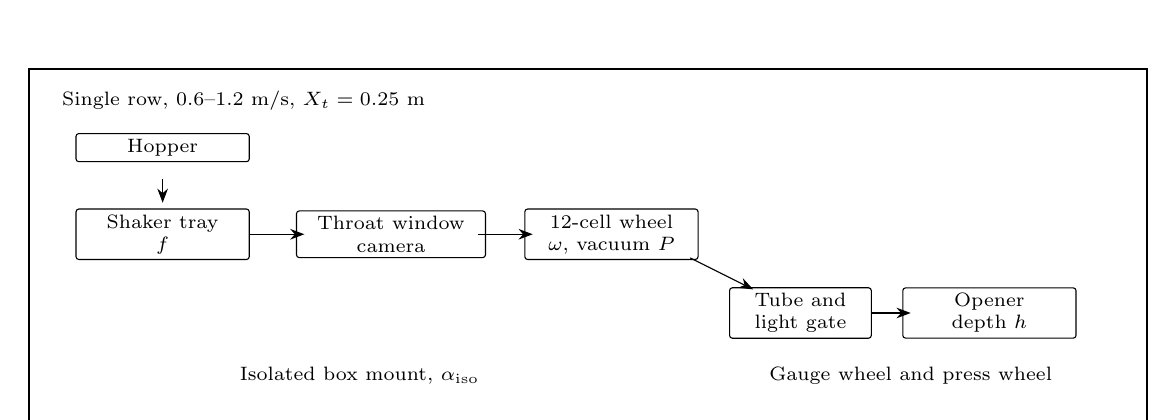
\begin{tikzpicture}[
  font=\scriptsize,
  box/.style={draw, rounded corners=1pt, align=center, inner sep=2pt},
  arr/.style={-{Stealth[length=1.8mm]}, thin}
]
\draw[thick] (0,0) rectangle (14.2,4.6);
\node[box, minimum width=22mm] at (1.7,3.6) {Hopper};
\node[box, minimum width=22mm] at (1.7,2.5) {Shaker tray\\$f$};
\node[box, minimum width=24mm] at (4.6,2.5) {Throat window\\camera};
\node[box, minimum width=22mm] at (7.4,2.5) {12-cell wheel\\$\omega$, vacuum $P$};
\node[box, minimum width=18mm] at (9.8,1.5) {Tube and\\light gate};
\node[box, minimum width=22mm] at (12.2,1.5) {Opener\\depth $h$};
\draw[arr] (1.7,3.2) -- (1.7,2.9);
\draw[arr] (2.8,2.5) -- (3.5,2.5);
\draw[arr] (5.7,2.5) -- (6.4,2.5);
\draw[arr] (8.4,2.2) -- (9.2,1.8);
\draw[arr] (10.7,1.5) -- (11.2,1.5);
\node[align=left] at (4.2,0.7) {Isolated box mount, $\alpha_{\mathrm{iso}}$};
\node[align=left] at (11.2,0.7) {Gauge wheel and press wheel};
\node[align=left, anchor=west] at (0.3,4.2) {Single row, 0.6--1.2~m/s, $X_t=0.25$~m};
\end{tikzpicture}
\caption{Seed path assumed by the controllers. Only frequency, vacuum, wheel speed, and depth are commands. The light gate counts seeds after release.}
\label{fig:machine}
\end{figure}

\subsection{Sensor list and what each signal is allowed to do}

Table~\ref{tab:sensors} is the interface control document in miniature. A signal that is not in the table does not enter a control law in this design. Adding a signal later is a revision, not a silent improvement, because the estimation will not have seen it.

\begin{table}[htbp]
\centering
\caption{Sensors, rates, and the loop allowed to consume each signal.}
\label{tab:sensors}
\begin{tabular}{@{}p{32mm}p{22mm}p{28mm}p{55mm}@{}}
\toprule
Sensor & Period & Consumer & Use \\
\midrule
Radar or undriven-wheel encoder & 10~ms & Feed loop & Ground speed $v$ in the kinematic law \\
Cell-wheel encoder & 10~ms & Feed loop & Shaft speed $\omega$ for the fuzzy PID \\
Throat camera & 50~ms & Vision computer & Features $\bar d$, $c_d$, $\rho$, $B$ \\
Tube light gate & event & Logger only & Delivered-rate estimate, not the constraint \\
Opener potentiometer & 10~ms & Depth servo & Hold $h^{\star}=30$~mm \\
Inertial unit on the frame & 20~ms & Factor loop & Dominant terrain frequency $f_{\mathrm{dist}}$ \\
Shaker current & 10~ms & Shaker amplifier & Track the frequency command \\
Vacuum transducer & 20~ms & Regulator & Track $P$, including the zero point \\
Hopper load cell & 100~ms & Logger only & Refill warning below 15 percent mass \\
\bottomrule
\end{tabular}
\end{table}

The inertial unit is not a navigation system. A short Fourier magnitude, updated every 200~ms on a one-second window of vertical acceleration, supplies the peak frequency inside 2 to 30~Hz. That peak is $f_{\mathrm{dist}}$ in Equation~\eqref{eq:feff}. If the spectrum is flat, the factor loop uses the last peak and sets a stale flag. A stale disturbance frequency freezes the frequency command and still allows vacuum to be optimised, because vacuum does not depend on $f_{\mathrm{eff}}$ except through the shared cost.

The camera calibration is a scale factor from pixels to millimetres, obtained from a 20~mm disk placed in the throat. Equivalent diameter in Equation~\eqref{eq:deq} inherits that scale. A 5 percent scale error moves a 20~mm seed by 1~mm, which is small beside the gap between pin oak and bur oak and is large beside a claim of millimetre metrology. The design does not make a millimetre claim. It claims that the bridge index rank-orders a packed throat against a flowing one.

\subsection{Computers and the bus between them}

Two processors are specified, matching the deadline split.

The feed computer is a small microcontroller with a hardware encoder interface and a 10~ms timer interrupt that cannot be disabled by the communication routine. It runs Equation~\eqref{eq:pid} and Equation~\eqref{eq:sigma}. It receives feature datagrams and factor-health bits. It does not decode images. Its worst-case execution for the control step is required to be under 2~ms, leaving 8~ms of idle time inside the period. That idle time is the margin Borja's combined processor did not have \cite{borja2021}.

The vision and factor computer is a single-board processor with a camera interface. Vision and the grid search share it because both are slow relative to the motor and both tolerate a missed deadline. They do not share a thread. Vision is a high-priority periodic thread at 50~ms. The grid search is a lower-priority thread released every 200~ms. If the search is still running when the next vision frame is due, the frame runs and the search continues. If the search is still running at the next 200~ms boundary, its result is discarded and the previous $(f,P)$ is held. Discarding a late result is safer than applying a result computed from a stale $\bar d$ that has since been replaced. The search was sized at 55 costs so that a discard is a fault, not the normal path.

The datagram between the boards is a fixed 32-byte record: time stamp, $\bar d$, $c_d$, $\rho$, $B$, vision-health, factor-health, $f$, $P$, and a checksum. A failed checksum is treated as a missed vision frame and follows the hold-and-decay rule. There is no dynamic allocation in the receive path. An ISO~11783 implement bus can carry the spacing set-point $X_t$ from a tractor terminal in a later integration \cite{iso11783}. The control laws do not read that bus in the design scored here. $X_t$ is a stored parameter.

Power is a 12~V machine bus with a separate regulator for the cameras and processors, so that a shaker current spike does not brown out the microcontroller. The shaker amplifier and the wheel motor have their own drivers and their own current limits. The wheel-motor current limit is set so that a jammed cell stalls the motor and raises the encoder-loss fault, rather than shearing the elastomer. That current limit is a mechanical-protection setting. It is not a control gain.

\subsection{Software tasks}

The tasks and their budgets are listed in Table~\ref{tab:tasks}. Budgets are requirements on a future implementation. They are consistent with the periods in Table~\ref{tab:params}. They have not been measured on a board in this study.

\begin{table}[htbp]
\centering
\caption{Tasks, periods, and the action on a missed deadline.}
\label{tab:tasks}
\begin{tabular}{@{}p{38mm}p{18mm}p{28mm}p{58mm}@{}}
\toprule
Task & Period & Budget & On a missed deadline \\
\midrule
Motor control & 10~ms & 2~ms & Stop the wheel if two periods are missed \\
Vision features & 50~ms & 30~ms & Feed loop holds $B$, then decays it \\
Depth servo & 10~ms & 1~ms & Hold last valve or motor command for 50~ms, then freeze depth \\
Disturbance spectrum & 200~ms & 20~ms & Freeze $f$, continue vacuum search \\
Factor grid & 200~ms & 40~ms & Keep previous feasible $(f,P)$ \\
Logger & 100~ms & 10~ms & Drop the oldest log block \\
\bottomrule
\end{tabular}
\end{table}

The logger is the only task allowed to drop data. Control tasks hold a feasible command or they stop the actuator. This is the operational content of requirement~9 in Section~\ref{sec:problem}. It is also the reason the factor search was not placed inside the motor interrupt. An occasional 40~ms search is acceptable on its own core and unacceptable inside a 10~ms interrupt.

State machines for the feed faults were listed in Section~\ref{sec:visiondesign}. The factor task adds two states. In \emph{search}, it publishes a new grid minimiser after the slew limit. In \emph{hold}, it publishes the previous command and lights a lamp. Entry to \emph{hold} is a late search, a stale $\bar d$ older than 500~ms, or a wheel-stopped bit from the feed computer. Exit from \emph{hold} requires three healthy cycles, so a flickering health bit does not chatter the shaker.

\subsection{Calibration procedure}

Calibration is a procedure, not a learning algorithm. It is specified because the features and the depth servo are meaningless without it. The order matters. A scale factor computed before the camera is clamped will be repeated after the next service and will silently shift $B$.

\begin{enumerate}
\item Clamp the camera and the lamp. Place the 20~mm disk in the throat on the centreline. Record the equivalent diameter reported by Equation~\eqref{eq:deq} and set the millimetre scale so that the report is 20~mm. Repeat at 10~mm left and right of centre. Reject the mount if the three reports differ by more than 0.6~mm.
\item Empty the throat. Record the residual image used by the background subtraction. Confirm that occupancy reads below 0.02.
\item Command the wheel at 15~r/min with an empty throat. The shaft encoder and a hand tachometer shall agree within 0.3~r/min. This checks Equation~\eqref{eq:wstar2}'s sensor, not the seed path.
\item Command $f$ from 2 to 12~Hz in 2~Hz steps against a strobe or a frequency output of the amplifier. The inertial unit, mounted for this step on the tray rather than on the frame, shall report the same peak within 0.5~Hz. Then return the unit to the frame.
\item Command $P$ at 0, 2, and 5~kPa. The transducer shall read within 0.3~kPa. The zero command shall read below 0.2~kPa. A zero that actually holds 1~kPa will bias the cost toward doubles on small seeds.
\item Set the opener on a flat rail and command 20, 30, and 40~mm. The potentiometer reading shall be within 1.5~mm. This is the sensor error. The 1.2~mm standard deviation used in the estimation is the closed-loop residual about the set-point, which includes rail roughness in the model and is not the same number as the calibration tolerance.
\item Drive the unit on a hard surface at a constant 1.0~m/s and compare radar speed with distance over time. The mean error shall be below 2 percent. Slip of a driven wheel is not a failure of this check. A difference between radar and the driven wheel is the slip the control law is there to ignore.
\end{enumerate}

No seed is required for these steps. A seed check is a bench experiment and sits outside this manuscript. The estimation does not use the tolerances as random errors except for the depth residual and the slip model already stated. Adding the calibration tolerances as extra noise would be a straightforward sensitivity run. It was not the run reported below.

\subsection{Safety interlocks}

The wheel motor is disabled when the opener is raised, so that a headland turn does not drill seeds onto the surface. The shaker is disabled when the hopper mass is below the refill threshold, so that an empty tray is not driven at 10~Hz for a bout. The vacuum pump or regulator is disabled at the same time. These interlocks are combinational logic on the feed computer, independent of the factor search. A software fault in $J$ cannot leave the shaker running on an empty machine once the load cell has crossed the threshold. The load cell itself can fail. A stuck high reading leaves the shaker enabled, which is the worse direction for noise and the safer direction for not silencing a full hopper. The failure is detected by the operator from the mass display, not by a second estimator.

\section{Estimation}
\label{sec:estimation}

\subsection{What is being estimated}

The estimation integrates the event model of Section~\ref{sec:predmodel} over long sequences of seeds. It asks how the indices move when the feed law and the factor law are switched on and off. The plant and the coordinator's predictor are the same logistic map. The Monte Carlo still has private randomness: each event draws a diameter from the lot, a slip, and a depth error. The coordinator sees only the lot mean and coefficient of variation. The feed constraint sees a filtered occupancy state, not the next diameter. The comparison is therefore a comparison of information and of actions, not a replay of one open-loop trajectory.

Five modes are defined.

\begin{enumerate}
\item \textbf{Ground.} The wheel is geared to the driven wheel. The speed scale equals $1-s$. Slip has mean $0.07+0.012$ times slope in degrees. Factors are fixed at $f=0$, $P=3$~kPa, and a passive depth error of standard deviation 6.5~mm. Terrain enters with $\alpha_{\mathrm{iso}}=1$.
\item \textbf{PID.} Electronic tracking of $\omega^{\star}$ from radar speed. The scale is 1 plus a small tracking residual of standard deviation 0.012. No vision constraint. Factors remain at the ground-drive constants. Slip is rejected except for a quarter of the ground-drive slip passed into the probability map, representing residual speed error.
\item \textbf{Vision.} The PID mode plus the bridge constraint of Equation~\eqref{eq:sigma}. Factors remain fixed. This mode is the first innovation alone.
\item \textbf{MPC.} The PID mode plus the grid minimiser of Equation~\eqref{eq:cost}, the isolated mount $\alpha_{\mathrm{iso}}=0.55$, and the tight depth residual of standard deviation 1.2~mm. Vision is off. This mode is the second innovation alone.
\item \textbf{Both.} Vision and MPC together.
\end{enumerate}

Each case runs 4{,}000 cell events. The random generator is the NumPy generator with seed 20261029 for the main table, and with seeds $20261029+17r$ for twelve repeats of the mixed-lot gain. The script that implements the modes is \texttt{simulate\_estimation.py}, stored with this manuscript. A reimplementation that follows Section~\ref{sec:predmodel} and the mode list above should match the table to sampling error. The script is the definition of the sampling error that was actually used.

Lots are log-normal in diameter. Pin oak has mean 15~mm and coefficient of variation 0.12. Red oak has 20.5~mm and 0.15. Bur oak has 32~mm and 0.20. The mixed lot has 22~mm and 0.32, which is a stand-in for a hopper that was not cleaned between species. Scenarios cross these lots with speed, slope, and a terrain frequency. The eight scenarios are the rows of the tables in this section. They were chosen to probe the requirements: a mild red-oak baseline, a slope, a harsh vibration, a small seed, a large seed, and a mixture.

Indices follow Equations~\eqref{eq:imult}--\eqref{eq:eta}. Positions are accumulated by advancing $X_t/\sigma$ at each event, placing one seed on a single, placing two seeds 0.22$X_t$ apart on a double, and placing nothing on a miss. Scatter from Equation~\eqref{eq:sigma_scatter} is added to the placed positions. Spacings are the positive differences of the sorted positions. This construction is how a miss becomes a gap near $2X_t$ and a double becomes a short gap, which is what the Kachman indices count \cite{kachman1995,iso7256}.

\subsection{Mild red oak}

Table~\ref{tab:redmild} gives red oak at 1.10~m/s, no slope, and a 6~Hz terrain disturbance. This is the easiest hardwood case that is still not a maize case. The cell is only slightly large for the seed.

\begin{table}[htbp]
\centering
\caption{Red oak, $v=1.10$~m/s, level ground, terrain frequency 6~Hz. Energy is the mean per event of $0.08\omega^2+0.012 f^2+0.02 P^2$ in the units of the script.}
\label{tab:redmild}
\begin{tabular}{@{}lrrrrrrr@{}}
\toprule
Mode & $Q_{\mathrm{f}}$ & $I_{\mathrm{mult}}$ & $I_{\mathrm{miss}}$ & $C_{\mathrm{v}}$ & $\eta_{\mathrm{E}}$ & Energy \\
\midrule
Ground & 58.58 & 21.65 & 19.78 & 20.13 & 52.38 & 0.55 \\
PID & 60.89 & 22.50 & 16.61 & 21.20 & 60.97 & 0.60 \\
Vision & 68.51 & 12.52 & 18.97 & 17.85 & 60.70 & 0.60 \\
MPC & 77.11 & 11.96 & 10.93 & 16.00 & 76.56 & 1.40 \\
Both & 88.20 & 5.59 & 6.22 & 12.88 & 87.00 & 1.39 \\
\bottomrule
\end{tabular}
\end{table}

Reading down the table is the answer to the three research questions for this scenario. The PID mode, which only rejects slip, moves the miss index from 19.8 to 16.6 percent and moves efficiency from 52.4 to 61.0 percent. It does nothing for doubles. The multiple index stays near 22 percent because the fixed 3~kPa vacuum and the slightly large cell are still there. Vision cuts the multiple index from 22.5 to 12.5 percent and raises quality of feed from 60.9 to 68.5 percent. Efficiency does not follow. It stays at 60.7 percent, because some of the seeds that are no longer doubled become stretched spacings and are counted as misses. The miss index rises from 16.6 to 19.0 percent. That rise is the interference the problem statement asked to be kept visible. On this mild case it cancels the productivity gain of vision and leaves the quality gain.

The factor coordinator is the large step. With vision still off, quality of feed reaches 77.1 percent, the miss index falls to 10.9 percent, and efficiency reaches 76.6 percent. The grid selects $f=9$~Hz and $P=0$. Zero vacuum is the map refusing the cereal habit. Nine hertz is the preferred agitation for a 20.5~mm seed, and with isolation the effective frequency stays under the 10~Hz anchor. Energy rises from 0.60 to 1.40 because the shaker is doing the work the vacuum is no longer doing. Stacking vision on top of that regime cuts the multiple index further, from 12.0 to 5.6 percent, and cuts the miss index as well, from 10.9 to 6.2 percent. Efficiency reaches 87.0 percent. On a regime the coordinator has already made flow, the constraint is active less often in a damaging way, and the two loops agree. Precision stays between 13 and 21 percent in every mode, inside the 30 percent band. Precision is not the term that separates these designs. Misses and doubles are.

The same lot at 0.70~m/s, still level, still at 6~Hz, is close to the 1.10~m/s table. Ground-drive quality of feed is 58.0 percent and efficiency is 51.5 percent. Both-mode quality of feed is 88.2 percent and efficiency is 87.3 percent. Speed, inside this narrow band, is not the main effect. Liu and colleagues found a clear speed effect on maize meters at field speeds well above this band \cite{liu2017speed}. The model does not add a further speed penalty beyond the scale error, so it should not be cited as a prediction of high-speed hardwood planting. The machine was never specified for that speed.

\begin{figure}[htbp]
\centering
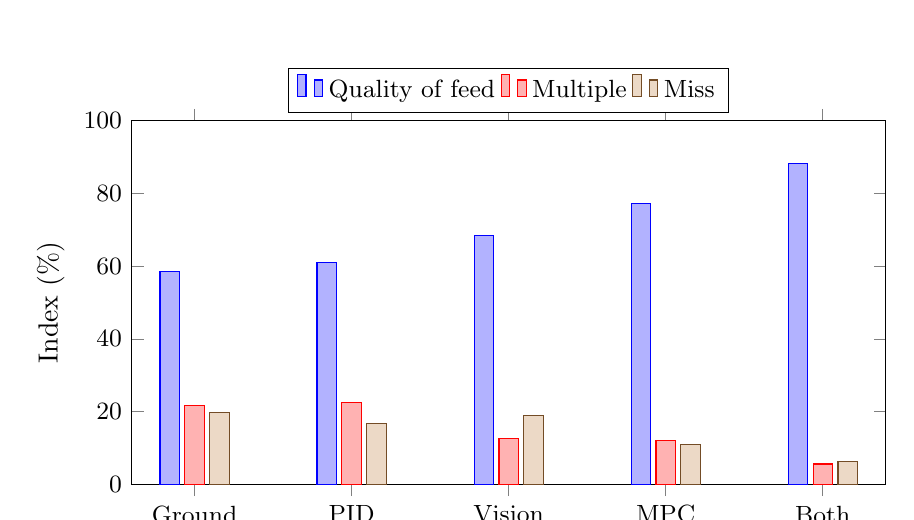
\begin{tikzpicture}
\begin{axis}[
  width=0.92\textwidth, height=6.2cm,
  ybar, bar width=7pt,
  ylabel={Index (\%)},
  symbolic x coords={Ground,PID,Vision,MPC,Both},
  xtick=data,
  ymin=0, ymax=100,
  legend style={font=\small, at={(0.5,1.02)}, anchor=south, legend columns=3},
  tick label style={font=\small}
]
\addplot coordinates {(Ground,58.58) (PID,60.89) (Vision,68.51) (MPC,77.11) (Both,88.20)};
\addplot coordinates {(Ground,21.65) (PID,22.50) (Vision,12.52) (MPC,11.96) (Both,5.59)};
\addplot coordinates {(Ground,19.78) (PID,16.61) (Vision,18.97) (MPC,10.93) (Both,6.22)};
\legend{Quality of feed, Multiple, Miss}
\end{axis}
\end{tikzpicture}
\caption{Red oak on level ground at 1.10~m/s. Vision trades a lower multiple index against a slightly higher miss index. The stacked system lowers both.}
\label{fig:redbars}
\end{figure}

\subsection{Slope and harsh vibration on red oak}

Slope is where the electronic drive earns its keep and where vision adds little. At 1.10~m/s and 12 degrees, with terrain still at 6~Hz, ground-drive quality of feed falls to 46.3 percent and efficiency falls to 28.9 percent. The miss index is 32.8 percent. Slip has stretched the spacing and the probability map has added misses. The PID mode returns the row to the level-ground electronic result: quality of feed 60.6 percent, efficiency 60.5 percent, miss index 17.2 percent. Vision reaches 68.5 percent quality of feed. MPC reaches 77.3 percent. Both reaches 88.2 percent quality of feed and 87.1 percent efficiency. Once slip is removed, the slope case and the level case are the same case. That is a property of the model, because slope enters only through slip. A real opener would also see a change of draft on a slope. The build logs draft and does not control it. The estimation therefore has nothing honest to add about draft.

Harsh vibration is a different disturbance. Table~\ref{tab:harsh} raises the terrain frequency to 16~Hz on level ground at 1.10~m/s, still with red oak.

\begin{table}[htbp]
\centering
\caption{Red oak, $v=1.10$~m/s, level ground, terrain frequency 16~Hz.}
\label{tab:harsh}
\begin{tabular}{@{}lrrrrrr@{}}
\toprule
Mode & $Q_{\mathrm{f}}$ & $I_{\mathrm{mult}}$ & $I_{\mathrm{miss}}$ & $C_{\mathrm{v}}$ & $\eta_{\mathrm{E}}$ & $f$ (Hz) \\
\midrule
Ground & 34.47 & 20.94 & 44.59 & 22.64 & 17.11 & 0 \\
PID & 36.94 & 21.20 & 41.86 & 24.24 & 21.77 & 0 \\
Vision & 41.12 & 13.24 & 45.64 & 21.89 & 21.99 & 0 \\
MPC & 67.16 & 16.28 & 16.56 & 18.80 & 64.46 & 3 \\
Both & 72.68 & 9.70 & 17.62 & 16.11 & 64.28 & 3 \\
\bottomrule
\end{tabular}
\end{table}

Shaft-speed tracking barely moves the miss index, from 44.6 to 41.9 percent. The seeds are being shaken out of the fill, and the shaft is not the cause. Vision lowers doubles from 21.2 to 13.2 percent and raises misses from 41.9 to 45.6 percent. Efficiency stays near 22 percent. Slowing a meter that is already missing because of vibration creates longer gaps. This is the clearest negative result for the first innovation used alone. It matches the design warning: the constraint is not a substitute for a bad factor regime.

The coordinator drops the shaker command from the 9~Hz of the mild case to 3~Hz. With $\alpha_{\mathrm{iso}}=0.55$, a 16~Hz terrain contribution and a 3~Hz command give an effective frequency near $\sqrt{(0.55\cdot 16)^2+3^2}\approx 9.3$~Hz, just under the harshness anchor. The miss index falls to 16.6 percent and efficiency rises to 64.5 percent. Energy per event falls to 0.53, below the PID mode's 0.60, because the optimiser has chosen the quiet command. Stacking vision raises quality of feed from 67.2 to 72.7 percent and cuts doubles from 16.3 to 9.7 percent, but efficiency does not rise. It is 64.3 percent. The extra quality is real and the extra planting rate is not, because the constraint still stretches some spacings. A user who cares about $Q_{\mathrm{f}}$ turns both loops on. A user who cares only about $\eta_{\mathrm{E}}$ under a 16~Hz disturbance gets essentially the whole gain from the factor loop and the isolator.

The 3~Hz choice is not a rule written for 16~Hz. It is the grid minimum of Equation~\eqref{eq:cost}. Neighbouring commands at 2~Hz and 4~Hz were available and lost. This is the behaviour required by requirement~8.

\subsection{Pin oak and the multiple index}

Pin oak at 15~mm is the small-seed requirement. At 1.10~m/s, level, 6~Hz terrain, ground drive posts a multiple index of 33.7 percent, a miss index of 15.7 percent, and a quality of feed of 50.6 percent. The cell is simply large. PID tracking leaves the multiple index at 34.3 percent and raises efficiency from 54.9 to 61.6 percent by removing slip. Vision cuts multiples to 24.3 percent and raises quality of feed to 60.6 percent. Efficiency moves only to 63.8 percent. The first innovation helps, and it does not repair a 9~mm mismatch by itself.

The coordinator selects 10~Hz and again 0~kPa. Quality of feed rises to 70.0 percent and the multiple index falls to 19.4 percent. Both loops together reach a multiple index of 10.3 percent, a miss index of 6.3 percent, a quality of feed of 83.4 percent, and an efficiency of 86.5 percent. The stack is worth more here than it was under harsh vibration. Small seeds double because of geometry and vacuum. Vision sees the irregular occupancy that goes with doubles, and the coordinator has removed the vacuum that was causing them. Each loop's action is aimed at the same error, so they add.

Ten hertz is at the top of the preferred-frequency curve for a 15~mm seed after the clip at 11~Hz. The cost is willing to sit next to the harshness anchor when the terrain itself is only 6~Hz and isolation is on. It is not willing to add 16~kPa, or 50~Hz, which is the vegetable-seed operating point \cite{li2025drum}. The grid's upper pressure is 5~kPa and the optimum is 0. Within the model, assist vacuum is the wrong tool for this cell and this lot.

\subsection{Bur oak and the miss index}

Bur oak is the Wells failure mode, put into the same table as the other lots \cite{wells1990}. The mean diameter is 32~mm against a 24~mm cell. No controller grows the cell. The question is how much of the miss index is recovered by time and by agitation.

At 0.70~m/s, level, 6~Hz, ground drive has a quality of feed of 34.5 percent, a miss index of 52.3 percent, and an efficiency of 14.8 percent. PID moves these to 37.2, 50.3, and 18.4. Vision moves quality of feed to 40.7 percent and efficiency to 16.9 percent, with the miss index still at 53.5 percent. Slowing the wheel without a better fill does not place large seeds. It waits longer between failures.

The coordinator selects 8~Hz and 0~kPa. Quality of feed rises to 63.1 percent, the miss index falls to 30.0 percent, and efficiency rises to 45.6 percent. Both loops reach 76.9 percent quality of feed, a miss index of 19.8 percent, a multiple index of 3.3 percent, and an efficiency of 57.9 percent. The residual miss index near 20 percent is the honest limit of a 24~mm cell on a 32~mm seed inside this map. The design does not claim a maize-grade meter on bur oak. It claims a large recovery relative to ground drive, and the table supports that claim inside the model: the miss index is cut by more than half, and efficiency rises from 15 percent to 58 percent.

The harsher bur-oak scenario adds an 8 degree slope and a 12~Hz terrain frequency at 1.10~m/s. Ground drive collapses to a quality of feed of 20.7 percent, a miss index of 66.5 percent, and an efficiency of 5.0 percent. PID recovers efficiency only to 11.9 percent. Vision, alone, sits at 9.8 percent efficiency with a miss index of 64.1 percent. MPC reaches 61.3 percent quality of feed and 44.0 percent efficiency at 7~Hz and 0~kPa. Both reaches 75.4 percent quality of feed, a miss index of 21.5 percent, and an efficiency of 55.1 percent. The first innovation is not useless in the stack. It is useless as a remedy for this disturbance by itself. That sentence is the practical output of the estimation for an implementer who might otherwise ship the camera and leave the shaker at the factory setting.

\begin{figure}[htbp]
\centering
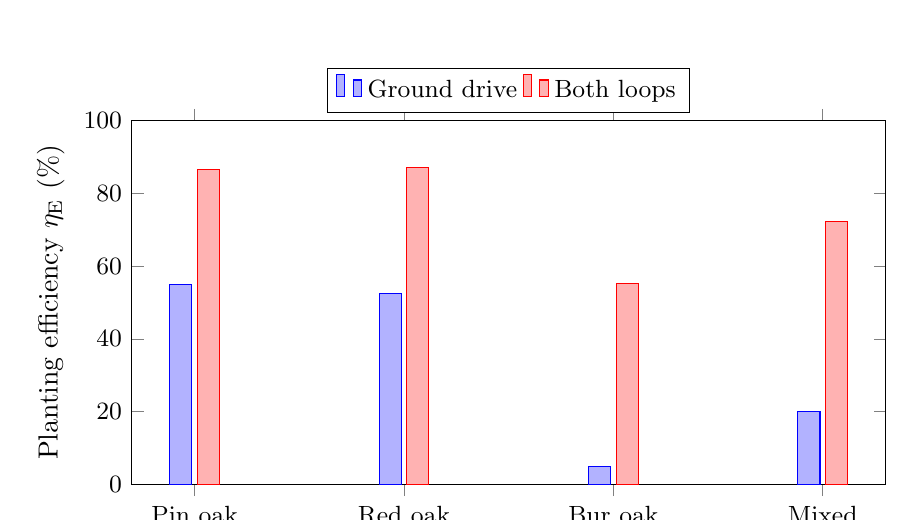
\begin{tikzpicture}
\begin{axis}[
  width=0.92\textwidth, height=6.2cm,
  ybar, bar width=8pt,
  ylabel={Planting efficiency $\eta_{\mathrm{E}}$ (\%)},
  symbolic x coords={Pin oak, Red oak, Bur oak, Mixed},
  xtick=data,
  ymin=0, ymax=100,
  legend style={font=\small, at={(0.5,1.02)}, anchor=south, legend columns=2},
  tick label style={font=\small},
  x tick label style={font=\small}
]
\addplot coordinates {(Pin oak,54.87) (Red oak,52.38) (Bur oak,5.01) (Mixed,20.12)};
\addplot coordinates {(Pin oak,86.49) (Red oak,87.00) (Bur oak,55.12) (Mixed,72.25)};
\legend{Ground drive, Both loops}
\end{axis}
\end{tikzpicture}
\caption{Planting efficiency of ground drive against both loops. Pin oak and red oak are the mild electronic cases at 1.10~m/s. Bur oak and the mixed lot include slope and a terrain frequency of 12~Hz. The bur-oak bar remains the lowest of the stacked results, which is the large-seed limit of a 24~mm cell.}
\label{fig:compare}
\end{figure}

\subsection{Mixed lot}

The mixed lot combines a 22~mm mean with a coefficient of variation of 0.32, an 8 degree slope, and a 12~Hz disturbance, at 1.10~m/s. It is the scenario in which a single fixed setup is least defensible. Ground drive scores 36.9 percent quality of feed, 24.0 percent multiples, 39.1 percent misses, and 20.1 percent efficiency. PID raises efficiency to 37.8 percent by rejecting slip and leaves multiples at 24.2 percent. Vision raises quality of feed to 50.4 percent, cuts multiples to 14.9 percent, and lowers efficiency to 33.5 percent. Again the constraint improves the composition of errors and gives back part of the rate.

MPC, at 8~Hz and 0~kPa, reaches 68.0 percent quality of feed and 65.2 percent efficiency. Both reaches 80.7 percent quality of feed, 7.6 percent multiples, 11.7 percent misses, precision 13.8 percent, and efficiency 72.3 percent. Twelve repeats of this one scenario, with different generator seeds, give a mean efficiency gain of the stacked system over ground drive of 50.8 percentage points, with a standard deviation of 0.89 points. The gain is stable across draws because 4{,}000 events is a long run. It is not stable across scenarios, and it should not be quoted as a universal 51-point improvement. On mild red oak the efficiency gain is $87.0-52.4=34.6$ points. On harsh red oak it is $64.3-17.1=47.2$ points. On the harsh bur-oak case it is $55.1-5.0=50.1$ points, from a very low base. The mixed-lot repeat only says that Monte Carlo noise is not the source of the ranking.

\subsection{Energy and the price terms}

Energy in the tables is not joules on a named motor. It is the mean per event of $0.08\omega^2 + 0.012 f^2 + 0.02 P^2$, evaluated in the script so that a faster wheel, a faster shaker, and a higher vacuum all cost something. Because the optimum vacuum is zero in every MPC row, the vacuum term does not drive the comparison. The shaker term does. Mild red oak at 9~Hz costs about 1.39 per event in the both-mode, against 0.60 for PID. Harsh red oak at 3~Hz costs 0.53, which is less than PID, because the wheel speed is similar and the shaker is quiet. The prices inside $J$ are what allow that quiet point to win when agitation would push $f_{\mathrm{eff}}$ over 10~Hz. If the prices were removed, the grid could still avoid 10~Hz through the harshness term in $z_m$. The prices matter for ties. They are not the sole reason the harsh-case command falls.

A deployer who is short of electrical power learns a specific lesson. The camera and the fuzzy loop are cheap in this energy proxy. The shaker is the cost of the second innovation, and it is a cost the optimiser already turns down when the frame is doing the shaking. Running the shaker at 9~Hz out of habit during a 16~Hz bout would pay the energy and, inside the model, would also pay in misses.

\subsection{Where the estimation can mislead}

Several readings would be stronger than the evidence.

The plant is the predictor. A coordinator that minimises $J$ on $\Pi$ will look good when the world is $\Pi$. The private randomness prevents a perfect score, and the tables show residual misses above 6 percent even in the best red-oak row, but a systematic error in the sign of a coefficient would move the real machine in the wrong direction while these tables stayed flattering. The coefficients most exposed to that risk are the 10~Hz anchor, which was observed on rapeseed \cite{zhang2024vib,wu2022}, and the isolator constant 0.55, which was not observed at all. A bench measurement of acorn fill against shaker frequency on this cell would replace both the anchor and the Gaussian width in Equation~\eqref{eq:agit}. Until that measurement exists, the ranking is a design calculation.

The camera is not simulated as an image. Occupancy is a filtered state driven by the rule in the script, not by rendered acorns. Occlusion, dust, and strobe failure are absent. The fault logic specifies what the software should do when features stop. It does not estimate how often they stop. Borja's accuracy on a clean plate, a fraction of a percent of frames wrong, is the optimistic reference \cite{borja2021}. A throat of wooden seeds is a harder image than a painted plate hole.

Depth noise is an independent Gaussian. Real depth error is correlated along the row, because the soil is correlated. Correlated error would widen the distribution of local spacing less than the independent model if the opener rides over a long wave, and it would create bursts of misses if the opener dives. The index means might move less than the appearance of a planted row. The estimation reports means.

Germination, rodent take, and the difference between a spacing and a surviving seedling are outside the indices by the scope statement \cite{lof2019,grossnickle2012}. A high $\eta_{\mathrm{E}}$ can still be a poor plantation. The machine-level claim stops at placement.

The ground-drive baseline uses $P=3$~kPa because that is a plausible leftover cereal setting, not because a hardwood manufacturer recommends it. Part of the MPC gain is the removal of a harmful default. If the baseline is redefined as $P=0$ and $f=0$ with electronic speed already on, the remaining gain is agitation, isolation, and depth, plus vision. That comparison is the PID-versus-MPC gap in the tables, not the ground-versus-both gap. On mild red oak it is $87.0-61.0=26.0$ efficiency points, still large, and it does not depend on accusing the ground drive of a bad vacuum. On that reading the PID row already has the bad vacuum. The MPC row removes it. The gain is still the factor decision.

\subsection{Answers to the research questions}

The questions in Section~\ref{sec:problem} can now be answered in the only sense this manuscript supports: as statements about the model.

The feed-speed loop with a vision constraint reduces doubles beyond shaft-speed tracking. On mild red oak the multiple index falls from 22.5 to 12.5 percent. On pin oak it falls from 34.3 to 24.3 percent. The same loop does not, by itself, reduce misses on bur oak or under a 16~Hz disturbance, and it can lower planting efficiency by stretching spacings. The first innovation is a quality intervention with a rate side effect. It should not be sold as a productivity controller.

The factor coordinator improves the indices in the regimes where tracking has little to offer. Under 16~Hz terrain the efficiency index moves from 21.8 percent with PID to 64.5 percent with the coordinator, at a lower shaker command. On harsh bur oak it moves from 11.9 percent to 44.0 percent before vision is added. The coordinator selects zero assist vacuum for every lot in the grid. Within the model, the right vacuum for this cell is none.

The loops interfere when the factor regime is bad, and they reinforce when the regime is good. Interference shows up as a quality gain without an efficiency gain: vision versus PID on mild red oak, and both versus MPC under 16~Hz. Reinforcement shows up as a gain in both indices: both versus MPC on pin oak, on bur oak, and on the mixed lot. The architecture did not make interference impossible. It made interference visible, because the two indices are published separately and because the coordinator is not allowed to assume that vision will hide its mistakes. That visibility is the system result. An implementer can turn the constraint off under a measured high terrain frequency and leave it on for a mixed or small-seed lot, using the same programs.

\subsection{What a bench would have to show}

A minimal bench, if one is built from Section~\ref{sec:build}, would need only enough instrumentation to recompute Table~\ref{tab:redmild} and Table~\ref{tab:harsh}. A sticky belt or a grease belt under the tube, a variable-speed belt under the wheels, and a shaker under the frame would reproduce the five modes \cite{panning2000,onal2009}. The acceptance test is not a single threshold. It is the ranking. Vision should cut the multiple index relative to PID on red oak and on pin oak. Vision alone should not be required to raise efficiency under a frame vibration above 10~Hz. The coordinator should select a low frequency in that case and a higher frequency when the frame is quiet. Both together should beat PID on bur oak by a margin large enough to see in a few hundred seeds, not only in 4{,}000. If the bench reverses the sign of the frequency effect, the Gaussian in Equation~\eqref{eq:agit} is the part to refit. The cascade structure, the deadline split, and the separation of $Q_{\mathrm{f}}$ from $\eta_{\mathrm{E}}$ would remain the parts worth keeping.

Until that belt is run, the numbers in this chapter are an estimate of a design, computed from a map that encodes the published failure modes of hardwood metering, of ground-wheel slip, of high-frequency vibration, and of a vision loop that slows the input of seeds. They are large enough, and consistent enough across lots, to justify the bench. They are not themselves the bench.

\subsection{The runs that were summarised}

Two red-oak runs and the slope run were described in prose so that the main tables would stay readable. They are recorded here at the same precision as Table~\ref{tab:redmild}, because a summary that cannot be checked against the script is not a result. Table~\ref{tab:rest} collects them. The both-mode frequency is 9~Hz and the vacuum is 0 in the slow and slope runs, and 3~Hz and 0 in the harsh run already discussed.

\begin{table}[htbp]
\centering
\caption{Remaining red-oak runs. Speed is in m/s, slope in degrees, terrain frequency in Hz.}
\label{tab:rest}
\begin{tabular}{@{}llrrrrr@{}}
\toprule
Case & Mode & $Q_{\mathrm{f}}$ & $I_{\mathrm{mult}}$ & $I_{\mathrm{miss}}$ & $C_{\mathrm{v}}$ & $\eta_{\mathrm{E}}$ \\
\midrule
0.70~m/s, 0$^\circ$, 6~Hz & Ground & 58.02 & 21.53 & 20.45 & 19.45 & 51.45 \\
 & PID & 60.24 & 21.35 & 18.41 & 21.44 & 59.48 \\
 & Vision & 65.58 & 13.27 & 21.16 & 18.12 & 57.41 \\
 & MPC & 77.49 & 12.09 & 10.42 & 16.11 & 77.68 \\
 & Both & 88.17 & 5.84 & 5.99 & 13.09 & 87.31 \\
\midrule
1.10~m/s, 12$^\circ$, 6~Hz & Ground & 46.34 & 20.87 & 32.79 & 17.57 & 28.89 \\
 & PID & 60.62 & 22.17 & 17.21 & 20.40 & 60.49 \\
 & Vision & 68.46 & 13.43 & 18.11 & 18.11 & 62.01 \\
 & MPC & 77.28 & 11.46 & 11.26 & 16.01 & 75.82 \\
 & Both & 88.22 & 5.61 & 6.17 & 12.57 & 87.05 \\
\bottomrule
\end{tabular}
\end{table}

The slow run repeats the mild-run pattern at a lower shaft speed. Vision lowers the multiple index from 21.4 to 13.3 percent and lowers efficiency from 59.5 to 57.4 percent. The rate side effect is visible even when the machine is already going slowly. MPC then both restore efficiency, to 77.7 and 87.3 percent. Nothing in the slow run suggests that the stack depends on the 1.10~m/s condition.

The slope run is the cleanest demonstration of requirement~2. Ground-drive efficiency is 28.9 percent with a miss index of 32.8 percent. Every electronic mode returns to within about one point of its level-ground efficiency at the same speed. The both-mode efficiency is 87.1 percent on the slope and 87.0 percent on the level. The model has no other slope channel. The table is what that modelling choice looks like when it is not smoothed into a sentence. A field trial in which electronic control failed to recover a slope would be evidence of a channel the model omitted, most likely opener draft, and not evidence that the arithmetic of Table~\ref{tab:rest} was mis-copied.

\subsection{Reading the near-tie under harsh vibration}

Section~\ref{sec:estimation} reported a 3~Hz command for red oak at 16~Hz terrain. The grid slice in Chapter~\ref{ch:design} shows why that command should not be over-interpreted. At the nominal diameter the predicted costs at 3~Hz and at 9~Hz differ by about $0.0001$. The drawn sample mean in the recorded run selected 3~Hz. Plant-side, with $\alpha_{\mathrm{iso}}=0.55$, a 3~Hz command and a 16~Hz terrain give $f_{\mathrm{eff}}\approx 9.3$~Hz, and a 9~Hz command would give about 12.6~Hz. The plant therefore experiences a real difference between the two commands even though the predictor, using the heavier weight 0.35 on $f_{\mathrm{dist}}^2$, scores them almost alike. The run that was printed used 3~Hz. A second run whose sample mean broke the tie the other way would print 9~Hz and would show a higher plant-side harshness. The efficiency gain over PID would remain, because both corners beat a command of 0~Hz, which is the PID and ground setting. The identity of the winning hertz would not remain. That is the correct confidence statement. The coordinator rejects the middle of the frequency range and rejects a non-zero vacuum. It does not, on this cost, identify a unique frequency once the terrain is already harsh.

\subsection{A note on repeatability of the other scenarios}

The twelve-repeat standard deviation of 0.89 points was computed only for the mixed-lot efficiency gain. The other scenarios were single runs of 4{,}000 events. A binomial picture of a proportion near 0.6 with 4{,}000 trials has a standard error near $\sqrt{0.6\cdot 0.4/4000}\approx 0.008$, or 0.8 percentage points, before the dependence among successive spacings is considered. Dependence widens the error. Doubling the binomial picture is a cautious reading: differences of two points in the tables are inside noise, and differences of ten points are not. The vision-versus-PID multiple-index drop on mild red oak is about ten points. The both-versus-ground efficiency gaps are tens of points. The vision-versus-PID efficiency differences of one point are not a finding. They were described as ``does not follow'' and ``stays'', which is the language that one point deserves.

The script seed is part of the result. A reader who changes the seed will move the fourth digit of a long run and can move the harsh-case frequency across the tie. Publishing the seed, 20261029, and the repeat rule $20261029+17r$, is what makes that movement a check rather than a contradiction. The file \texttt{estimation\_results.json} stores the run that the tables were typed from.

\subsection{Consolidated efficiency}

Table~\ref{tab:all} puts every scenario's planting efficiency on one page so that the ranking does not depend on which prose paragraph a reader happens to remember. The both-mode column is the stack. The ground column is the open-loop machine. The gap between them is the quantity the title of this manuscript refers to, and it is a model quantity.

\begin{table}[htbp]
\centering
\caption{Planting efficiency $\eta_{\mathrm{E}}$ in percent for every estimated scenario. Terrain frequency $f_{\mathrm{dist}}$ is in hertz and slope is in degrees. Speed is in m/s.}
\label{tab:all}
\begin{tabular}{@{}llrrrrr@{}}
\toprule
Lot & Condition & Ground & PID & Vision & MPC & Both \\
\midrule
Red oak & 0.70, 0$^\circ$, 6~Hz & 51.45 & 59.48 & 57.41 & 77.68 & 87.31 \\
Red oak & 1.10, 0$^\circ$, 6~Hz & 52.38 & 60.97 & 60.70 & 76.56 & 87.00 \\
Red oak & 1.10, 12$^\circ$, 6~Hz & 28.89 & 60.49 & 62.01 & 75.82 & 87.05 \\
Red oak & 1.10, 0$^\circ$, 16~Hz & 17.11 & 21.77 & 21.99 & 64.46 & 64.28 \\
Pin oak & 1.10, 0$^\circ$, 6~Hz & 54.87 & 61.61 & 63.78 & 75.20 & 86.49 \\
Bur oak & 0.70, 0$^\circ$, 6~Hz & 14.76 & 18.35 & 16.85 & 45.62 & 57.86 \\
Bur oak & 1.10, 8$^\circ$, 12~Hz & 5.01 & 11.93 & 9.82 & 43.99 & 55.12 \\
Mixed & 1.10, 8$^\circ$, 12~Hz & 20.12 & 37.75 & 33.52 & 65.19 & 72.25 \\
\bottomrule
\end{tabular}
\end{table}

The column order is the order in which a builder would add the pieces. PID recovers the slope row and little else. Vision, added to PID, does not dominate that column: it wins on pin oak and on the slope, and it loses a point or more on the slow red oak, on both bur-oak rows, and on the mixed lot. MPC, added instead of vision, wins every row against PID by a wide margin, and the margin is widest where the ground drive has collapsed. Both, added last, wins every row against MPC except the harsh red-oak row, where it is 0.18 points lower, inside the repeatability note above. The architecture's claim is not that the stack is uniformly better than its better half. The claim is that the better half is different in different rows, and that publishing both indices, of which this table shows only efficiency, keeps a builder from turning on a loop that the row does not need. On a harsh red-oak bout the factor loop is the one that pays. On a pin-oak bout the camera still earns its place, because the both-mode efficiency of 86.5 percent is eleven points above MPC. The table is the decision.




\bibliographystyle{unsrt}
\bibliography{refs}

\end{document}
